
\documentclass{article} % For LaTeX2e
\usepackage[table,xcdraw]{xcolor}

\usepackage{iclr2025_conference,times}

% Optional math commands from https://github.com/goodfeli/dlbook_notation.
%%%%% NEW MATH DEFINITIONS %%%%%

\usepackage{amsmath,amsfonts,bm}

% Mark sections of captions for referring to divisions of figures
\newcommand{\figleft}{{\em (Left)}}
\newcommand{\figcenter}{{\em (Center)}}
\newcommand{\figright}{{\em (Right)}}
\newcommand{\figtop}{{\em (Top)}}
\newcommand{\figbottom}{{\em (Bottom)}}
\newcommand{\captiona}{{\em (a)}}
\newcommand{\captionb}{{\em (b)}}
\newcommand{\captionc}{{\em (c)}}
\newcommand{\captiond}{{\em (d)}}

% Highlight a newly defined term
\newcommand{\newterm}[1]{{\bf #1}}


% Figure reference, lower-case.
\def\figref#1{figure~\ref{#1}}
% Figure reference, capital. For start of sentence
\def\Figref#1{Figure~\ref{#1}}
\def\twofigref#1#2{figures \ref{#1} and \ref{#2}}
\def\quadfigref#1#2#3#4{figures \ref{#1}, \ref{#2}, \ref{#3} and \ref{#4}}
% Section reference, lower-case.
\def\secref#1{section~\ref{#1}}
% Section reference, capital.
\def\Secref#1{Section~\ref{#1}}
% Reference to two sections.
\def\twosecrefs#1#2{sections \ref{#1} and \ref{#2}}
% Reference to three sections.
\def\secrefs#1#2#3{sections \ref{#1}, \ref{#2} and \ref{#3}}
% Reference to an equation, lower-case.
% \def\eqref#1{equation~\ref{#1}}
\def\eqref#1{(\ref{#1})}
% Reference to an equation, upper case
\def\Eqref#1{Equation~\ref{#1}}
% A raw reference to an equation---avoid using if possible
\def\plaineqref#1{\ref{#1}}
% Reference to a chapter, lower-case.
\def\chapref#1{chapter~\ref{#1}}
% Reference to an equation, upper case.
\def\Chapref#1{Chapter~\ref{#1}}
% Reference to a range of chapters
\def\rangechapref#1#2{chapters\ref{#1}--\ref{#2}}
% Reference to an algorithm, lower-case.
\def\algref#1{algorithm~\ref{#1}}
% Reference to an algorithm, upper case.
\def\Algref#1{Algorithm~\ref{#1}}
\def\twoalgref#1#2{algorithms \ref{#1} and \ref{#2}}
\def\Twoalgref#1#2{Algorithms \ref{#1} and \ref{#2}}
% Reference to a part, lower case
\def\partref#1{part~\ref{#1}}
% Reference to a part, upper case
\def\Partref#1{Part~\ref{#1}}
\def\twopartref#1#2{parts \ref{#1} and \ref{#2}}

\def\ceil#1{\lceil #1 \rceil}
\def\floor#1{\lfloor #1 \rfloor}
\def\1{\bm{1}}
\newcommand{\train}{\mathcal{D}}
\newcommand{\valid}{\mathcal{D_{\mathrm{valid}}}}
\newcommand{\test}{\mathcal{D_{\mathrm{test}}}}

\def\eps{{\epsilon}}


% Random variables
\def\reta{{\textnormal{$\eta$}}}
\def\ra{{\textnormal{a}}}
\def\rb{{\textnormal{b}}}
\def\rc{{\textnormal{c}}}
\def\rd{{\textnormal{d}}}
\def\re{{\textnormal{e}}}
\def\rf{{\textnormal{f}}}
\def\rg{{\textnormal{g}}}
\def\rh{{\textnormal{h}}}
\def\ri{{\textnormal{i}}}
\def\rj{{\textnormal{j}}}
\def\rk{{\textnormal{k}}}
\def\rl{{\textnormal{l}}}
% rm is already a command, just don't name any random variables m
\def\rn{{\textnormal{n}}}
\def\ro{{\textnormal{o}}}
\def\rp{{\textnormal{p}}}
\def\rq{{\textnormal{q}}}
\def\rr{{\textnormal{r}}}
\def\rs{{\textnormal{s}}}
\def\rt{{\textnormal{t}}}
\def\ru{{\textnormal{u}}}
\def\rv{{\textnormal{v}}}
\def\rw{{\textnormal{w}}}
\def\rx{{\textnormal{x}}}
\def\ry{{\textnormal{y}}}
\def\rz{{\textnormal{z}}}

% Random vectors
\def\rvepsilon{{\mathbf{\epsilon}}}
\def\rvtheta{{\mathbf{\theta}}}
\def\rva{{\mathbf{a}}}
\def\rvb{{\mathbf{b}}}
\def\rvc{{\mathbf{c}}}
\def\rvd{{\mathbf{d}}}
\def\rve{{\mathbf{e}}}
\def\rvf{{\mathbf{f}}}
\def\rvg{{\mathbf{g}}}
\def\rvh{{\mathbf{h}}}
\def\rvu{{\mathbf{i}}}
\def\rvj{{\mathbf{j}}}
\def\rvk{{\mathbf{k}}}
\def\rvl{{\mathbf{l}}}
\def\rvm{{\mathbf{m}}}
\def\rvn{{\mathbf{n}}}
\def\rvo{{\mathbf{o}}}
\def\rvp{{\mathbf{p}}}
\def\rvq{{\mathbf{q}}}
\def\rvr{{\mathbf{r}}}
\def\rvs{{\mathbf{s}}}
\def\rvt{{\mathbf{t}}}
\def\rvu{{\mathbf{u}}}
\def\rvv{{\mathbf{v}}}
\def\rvw{{\mathbf{w}}}
\def\rvx{{\mathbf{x}}}
\def\rvy{{\mathbf{y}}}
\def\rvz{{\mathbf{z}}}

% Elements of random vectors
\def\erva{{\textnormal{a}}}
\def\ervb{{\textnormal{b}}}
\def\ervc{{\textnormal{c}}}
\def\ervd{{\textnormal{d}}}
\def\erve{{\textnormal{e}}}
\def\ervf{{\textnormal{f}}}
\def\ervg{{\textnormal{g}}}
\def\ervh{{\textnormal{h}}}
\def\ervi{{\textnormal{i}}}
\def\ervj{{\textnormal{j}}}
\def\ervk{{\textnormal{k}}}
\def\ervl{{\textnormal{l}}}
\def\ervm{{\textnormal{m}}}
\def\ervn{{\textnormal{n}}}
\def\ervo{{\textnormal{o}}}
\def\ervp{{\textnormal{p}}}
\def\ervq{{\textnormal{q}}}
\def\ervr{{\textnormal{r}}}
\def\ervs{{\textnormal{s}}}
\def\ervt{{\textnormal{t}}}
\def\ervu{{\textnormal{u}}}
\def\ervv{{\textnormal{v}}}
\def\ervw{{\textnormal{w}}}
\def\ervx{{\textnormal{x}}}
\def\ervy{{\textnormal{y}}}
\def\ervz{{\textnormal{z}}}

% Random matrices
\def\rmA{{\mathbf{A}}}
\def\rmB{{\mathbf{B}}}
\def\rmC{{\mathbf{C}}}
\def\rmD{{\mathbf{D}}}
\def\rmE{{\mathbf{E}}}
\def\rmF{{\mathbf{F}}}
\def\rmG{{\mathbf{G}}}
\def\rmH{{\mathbf{H}}}
\def\rmI{{\mathbf{I}}}
\def\rmJ{{\mathbf{J}}}
\def\rmK{{\mathbf{K}}}
\def\rmL{{\mathbf{L}}}
\def\rmM{{\mathbf{M}}}
\def\rmN{{\mathbf{N}}}
\def\rmO{{\mathbf{O}}}
\def\rmP{{\mathbf{P}}}
\def\rmQ{{\mathbf{Q}}}
\def\rmR{{\mathbf{R}}}
\def\rmS{{\mathbf{S}}}
\def\rmT{{\mathbf{T}}}
\def\rmU{{\mathbf{U}}}
\def\rmV{{\mathbf{V}}}
\def\rmW{{\mathbf{W}}}
\def\rmX{{\mathbf{X}}}
\def\rmY{{\mathbf{Y}}}
\def\rmZ{{\mathbf{Z}}}

% Elements of random matrices
\def\ermA{{\textnormal{A}}}
\def\ermB{{\textnormal{B}}}
\def\ermC{{\textnormal{C}}}
\def\ermD{{\textnormal{D}}}
\def\ermE{{\textnormal{E}}}
\def\ermF{{\textnormal{F}}}
\def\ermG{{\textnormal{G}}}
\def\ermH{{\textnormal{H}}}
\def\ermI{{\textnormal{I}}}
\def\ermJ{{\textnormal{J}}}
\def\ermK{{\textnormal{K}}}
\def\ermL{{\textnormal{L}}}
\def\ermM{{\textnormal{M}}}
\def\ermN{{\textnormal{N}}}
\def\ermO{{\textnormal{O}}}
\def\ermP{{\textnormal{P}}}
\def\ermQ{{\textnormal{Q}}}
\def\ermR{{\textnormal{R}}}
\def\ermS{{\textnormal{S}}}
\def\ermT{{\textnormal{T}}}
\def\ermU{{\textnormal{U}}}
\def\ermV{{\textnormal{V}}}
\def\ermW{{\textnormal{W}}}
\def\ermX{{\textnormal{X}}}
\def\ermY{{\textnormal{Y}}}
\def\ermZ{{\textnormal{Z}}}

% Vectors
\def\vzero{{\bm{0}}}
\def\vone{{\bm{1}}}
\def\vmu{{\bm{\mu}}}
\def\vtheta{{\bm{\theta}}}
\def\va{{\bm{a}}}
\def\vb{{\bm{b}}}
\def\vc{{\bm{c}}}
\def\vd{{\bm{d}}}
\def\ve{{\bm{e}}}
\def\vf{{\bm{f}}}
\def\vg{{\bm{g}}}
\def\vh{{\bm{h}}}
\def\vi{{\bm{i}}}
\def\vj{{\bm{j}}}
\def\vk{{\bm{k}}}
\def\vl{{\bm{l}}}
\def\vm{{\bm{m}}}
\def\vn{{\bm{n}}}
\def\vo{{\bm{o}}}
\def\vp{{\bm{p}}}
\def\vq{{\bm{q}}}
\def\vr{{\bm{r}}}
\def\vs{{\bm{s}}}
\def\vt{{\bm{t}}}
\def\vu{{\bm{u}}}
\def\vv{{\bm{v}}}
\def\vw{{\bm{w}}}
\def\vx{{\bm{x}}}
\def\vy{{\bm{y}}}
\def\vz{{\bm{z}}}

% Elements of vectors
\def\evalpha{{\alpha}}
\def\evbeta{{\beta}}
\def\evepsilon{{\epsilon}}
\def\evlambda{{\lambda}}
\def\evomega{{\omega}}
\def\evmu{{\mu}}
\def\evpsi{{\psi}}
\def\evsigma{{\sigma}}
\def\evtheta{{\theta}}
\def\eva{{a}}
\def\evb{{b}}
\def\evc{{c}}
\def\evd{{d}}
\def\eve{{e}}
\def\evf{{f}}
\def\evg{{g}}
\def\evh{{h}}
\def\evi{{i}}
\def\evj{{j}}
\def\evk{{k}}
\def\evl{{l}}
\def\evm{{m}}
\def\evn{{n}}
\def\evo{{o}}
\def\evp{{p}}
\def\evq{{q}}
\def\evr{{r}}
\def\evs{{s}}
\def\evt{{t}}
\def\evu{{u}}
\def\evv{{v}}
\def\evw{{w}}
\def\evx{{x}}
\def\evy{{y}}
\def\evz{{z}}

% Matrix
\def\mA{{\bm{A}}}
\def\mB{{\bm{B}}}
\def\mC{{\bm{C}}}
\def\mD{{\bm{D}}}
\def\mE{{\bm{E}}}
\def\mF{{\bm{F}}}
\def\mG{{\bm{G}}}
\def\mH{{\bm{H}}}
\def\mI{{\bm{I}}}
\def\mJ{{\bm{J}}}
\def\mK{{\bm{K}}}
\def\mL{{\bm{L}}}
\def\mM{{\bm{M}}}
\def\mN{{\bm{N}}}
\def\mO{{\bm{O}}}
\def\mP{{\bm{P}}}
\def\mQ{{\bm{Q}}}
\def\mR{{\bm{R}}}
\def\mS{{\bm{S}}}
\def\mT{{\bm{T}}}
\def\mU{{\bm{U}}}
\def\mV{{\bm{V}}}
\def\mW{{\bm{W}}}
\def\mX{{\bm{X}}}
\def\mY{{\bm{Y}}}
\def\mZ{{\bm{Z}}}
\def\mBeta{{\bm{\beta}}}
\def\mPhi{{\bm{\Phi}}}
\def\mLambda{{\bm{\Lambda}}}
\def\mSigma{{\bm{\Sigma}}}

% Tensor
\DeclareMathAlphabet{\mathsfit}{\encodingdefault}{\sfdefault}{m}{sl}
\SetMathAlphabet{\mathsfit}{bold}{\encodingdefault}{\sfdefault}{bx}{n}
\newcommand{\tens}[1]{\bm{\mathsfit{#1}}}
\def\tA{{\tens{A}}}
\def\tB{{\tens{B}}}
\def\tC{{\tens{C}}}
\def\tD{{\tens{D}}}
\def\tE{{\tens{E}}}
\def\tF{{\tens{F}}}
\def\tG{{\tens{G}}}
\def\tH{{\tens{H}}}
\def\tI{{\tens{I}}}
\def\tJ{{\tens{J}}}
\def\tK{{\tens{K}}}
\def\tL{{\tens{L}}}
\def\tM{{\tens{M}}}
\def\tN{{\tens{N}}}
\def\tO{{\tens{O}}}
\def\tP{{\tens{P}}}
\def\tQ{{\tens{Q}}}
\def\tR{{\tens{R}}}
\def\tS{{\tens{S}}}
\def\tT{{\tens{T}}}
\def\tU{{\tens{U}}}
\def\tV{{\tens{V}}}
\def\tW{{\tens{W}}}
\def\tX{{\tens{X}}}
\def\tY{{\tens{Y}}}
\def\tZ{{\tens{Z}}}


% Graph
\def\gA{{\mathcal{A}}}
\def\gB{{\mathcal{B}}}
\def\gC{{\mathcal{C}}}
\def\gD{{\mathcal{D}}}
\def\gE{{\mathcal{E}}}
\def\gF{{\mathcal{F}}}
\def\gG{{\mathcal{G}}}
\def\gH{{\mathcal{H}}}
\def\gI{{\mathcal{I}}}
\def\gJ{{\mathcal{J}}}
\def\gK{{\mathcal{K}}}
\def\gL{{\mathcal{L}}}
\def\gM{{\mathcal{M}}}
\def\gN{{\mathcal{N}}}
\def\gO{{\mathcal{O}}}
\def\gP{{\mathcal{P}}}
\def\gQ{{\mathcal{Q}}}
\def\gR{{\mathcal{R}}}
\def\gS{{\mathcal{S}}}
\def\gT{{\mathcal{T}}}
\def\gU{{\mathcal{U}}}
\def\gV{{\mathcal{V}}}
\def\gW{{\mathcal{W}}}
\def\gX{{\mathcal{X}}}
\def\gY{{\mathcal{Y}}}
\def\gZ{{\mathcal{Z}}}

% Sets
\def\sA{{\mathbb{A}}}
\def\sB{{\mathbb{B}}}
\def\sC{{\mathbb{C}}}
\def\sD{{\mathbb{D}}}
% Don't use a set called E, because this would be the same as our symbol
% for expectation.
\def\sF{{\mathbb{F}}}
\def\sG{{\mathbb{G}}}
\def\sH{{\mathbb{H}}}
\def\sI{{\mathbb{I}}}
\def\sJ{{\mathbb{J}}}
\def\sK{{\mathbb{K}}}
\def\sL{{\mathbb{L}}}
\def\sM{{\mathbb{M}}}
\def\sN{{\mathbb{N}}}
\def\sO{{\mathbb{O}}}
\def\sP{{\mathbb{P}}}
\def\sQ{{\mathbb{Q}}}
\def\sR{{\mathbb{R}}}
\def\sS{{\mathbb{S}}}
\def\sT{{\mathbb{T}}}
\def\sU{{\mathbb{U}}}
\def\sV{{\mathbb{V}}}
\def\sW{{\mathbb{W}}}
\def\sX{{\mathbb{X}}}
\def\sY{{\mathbb{Y}}}
\def\sZ{{\mathbb{Z}}}

% Entries of a matrix
\def\emLambda{{\Lambda}}
\def\emA{{A}}
\def\emB{{B}}
\def\emC{{C}}
\def\emD{{D}}
\def\emE{{E}}
\def\emF{{F}}
\def\emG{{G}}
\def\emH{{H}}
\def\emI{{I}}
\def\emJ{{J}}
\def\emK{{K}}
\def\emL{{L}}
\def\emM{{M}}
\def\emN{{N}}
\def\emO{{O}}
\def\emP{{P}}
\def\emQ{{Q}}
\def\emR{{R}}
\def\emS{{S}}
\def\emT{{T}}
\def\emU{{U}}
\def\emV{{V}}
\def\emW{{W}}
\def\emX{{X}}
\def\emY{{Y}}
\def\emZ{{Z}}
\def\emSigma{{\Sigma}}

% entries of a tensor
% Same font as tensor, without \bm wrapper
\newcommand{\etens}[1]{\mathsfit{#1}}
\def\etLambda{{\etens{\Lambda}}}
\def\etA{{\etens{A}}}
\def\etB{{\etens{B}}}
\def\etC{{\etens{C}}}
\def\etD{{\etens{D}}}
\def\etE{{\etens{E}}}
\def\etF{{\etens{F}}}
\def\etG{{\etens{G}}}
\def\etH{{\etens{H}}}
\def\etI{{\etens{I}}}
\def\etJ{{\etens{J}}}
\def\etK{{\etens{K}}}
\def\etL{{\etens{L}}}
\def\etM{{\etens{M}}}
\def\etN{{\etens{N}}}
\def\etO{{\etens{O}}}
\def\etP{{\etens{P}}}
\def\etQ{{\etens{Q}}}
\def\etR{{\etens{R}}}
\def\etS{{\etens{S}}}
\def\etT{{\etens{T}}}
\def\etU{{\etens{U}}}
\def\etV{{\etens{V}}}
\def\etW{{\etens{W}}}
\def\etX{{\etens{X}}}
\def\etY{{\etens{Y}}}
\def\etZ{{\etens{Z}}}

% The true underlying data generating distribution
\newcommand{\pdata}{p_{\rm{data}}}
% The empirical distribution defined by the training set
\newcommand{\ptrain}{\hat{p}_{\rm{data}}}
\newcommand{\Ptrain}{\hat{P}_{\rm{data}}}
% The model distribution
\newcommand{\pmodel}{p_{\rm{model}}}
\newcommand{\Pmodel}{P_{\rm{model}}}
\newcommand{\ptildemodel}{\tilde{p}_{\rm{model}}}
% Stochastic autoencoder distributions
\newcommand{\pencode}{p_{\rm{encoder}}}
\newcommand{\pdecode}{p_{\rm{decoder}}}
\newcommand{\precons}{p_{\rm{reconstruct}}}

\newcommand{\laplace}{\mathrm{Laplace}} % Laplace distribution

\newcommand{\E}{\mathbb{E}}
\newcommand{\Ls}{\mathcal{L}}
\newcommand{\R}{\mathbb{R}}
\newcommand{\emp}{\tilde{p}}
\newcommand{\lr}{\alpha}
\newcommand{\reg}{\lambda}
\newcommand{\rect}{\mathrm{rectifier}}
\newcommand{\softmax}{\mathrm{softmax}}
\newcommand{\sigmoid}{\sigma}
\newcommand{\softplus}{\zeta}
\newcommand{\KL}{D_{\mathrm{KL}}}
\newcommand{\Var}{\mathrm{Var}}
\newcommand{\standarderror}{\mathrm{SE}}
\newcommand{\Cov}{\mathrm{Cov}}
% Wolfram Mathworld says $L^2$ is for function spaces and $\ell^2$ is for vectors
% But then they seem to use $L^2$ for vectors throughout the site, and so does
% wikipedia.
\newcommand{\normlzero}{L^0}
\newcommand{\normlone}{L^1}
\newcommand{\normltwo}{L^2}
\newcommand{\normlp}{L^p}
\newcommand{\normmax}{L^\infty}

\newcommand{\parents}{Pa} % See usage in notation.tex. Chosen to match Daphne's book.

\DeclareMathOperator*{\argmax}{arg\,max}
\DeclareMathOperator*{\argmin}{arg\,min}

\DeclareMathOperator{\sign}{sign}
\DeclareMathOperator{\Tr}{Tr}
\let\ab\allowbreak

\usepackage{hyperref}
\usepackage{booktabs}
\usepackage{multirow}
\usepackage{url}
% \usepackage[normalem]{ulem}
% \useunder{\uline}{\ul}{}
\usepackage{adjustbox}
\usepackage{wrapfig}
\usepackage{float}
\usepackage{dsfont}

\usepackage{amsmath}
\usepackage{enumitem}
\usepackage[capitalise,noabbrev]{cleveref}

% Define a custom dark blue color
\definecolor{darkblue}{rgb}{0.0, 0.0, 0.5}

% hyperref setup
\hypersetup{
    colorlinks=true,
    linkcolor=darkblue,      % Color for internal links (sections, pages)
    citecolor=darkblue,      % Color for citation links (bibliography)
    urlcolor=darkblue        % Color for external links (URLs)
}

\title{FLARE: Faithful Logic-Aided Reasoning and Exploration
}

% Authors must not appear in the submitted version. They should be hidden
% as long as the \iclrfinalcopy macro remains commented out below.
% Non-anonymous submissions will be rejected without review.

 \iclrfinalcopy

\newcommand\blfootnote[1]{%
  \begingroup
  \renewcommand\thefootnote{}\footnote{#1}%
  \addtocounter{footnote}{-1}%
  \endgroup
}

\author{%
Erik Arakelyan$^{\dagger1}$ \quad Pasquale Minervini$^{2}$$^{3}$ \quad Pat Verga$^4$ \quad Patrick Lewis$^4$ \quad Isabelle Augenstein$^1$ \\
$^1$University of Copenhagen \qquad $^2$University of Edinburgh \qquad $^3$Miniml.AI \qquad $^4$Cohere \\
\texttt{\{erik.a, augenstein\}@di.ku.dk} \qquad  \texttt{p.minervini@ed.ac.uk} \\ \texttt{\{pat, patrick\}@cohere.com}
}


% The \author macro works with any number of authors. There are two commands
% used to separate the names and addresses of multiple authors: \And and \AND.
%
% Using \And between authors leaves it to \LaTeX{} to determine where to break
% the lines. Using \AND forces a linebreak at that point. So, if \LaTeX{}
% puts 3 of 4 authors names on the first line, and the last on the second
% line, try using \AND instead of \And before the third author name.

\newcommand{\fix}{\marginpar{FIX}}
\newcommand{\new}{\marginpar{NEW}}
\newcommand{\ours}{\texorpdfstring{FLARE}\xspace}

%\iclrfinalcopy % Uncomment for camera-ready version, but NOT for submission.
\begin{document}


\maketitle

\blfootnote{$^{\dagger}$Corresponding author.}

\begin{abstract}
%
%Modern Question Answering (QA) and Reasoning benchmarks have favoured Large Language Models (LLMs) for their strong performance. Such models commonly utilise prompting techniques, such as Chain-of-Thought (CoT), assuming the resulting generation will have a more granular exploration and reasoning over the question space and scope.
%
Modern Question Answering (QA) and Reasoning approaches based on Large Language Models (LLMs) commonly use prompting techniques, such as Chain-of-Thought (CoT), assuming the resulting generation will have a more granular exploration and reasoning over the question space and scope.
%
However, such methods struggle with generating outputs that are faithful to the intermediate chain of reasoning produced by the model.
%
%On the other end of the spectrum, methods such as Faithful CoT (F-CoT) propose to use LLMs with symbolic methods to formalise the natural language text and produce a solution using a solver.
%
On the other end of the spectrum, neuro-symbolic methods such as Faithful CoT (F-CoT) propose to combine LLMs with external symbolic solvers.
%
While such approaches boast a high degree of faithfulness, they usually require a model trained for code generation and struggle with tasks that are ambiguous or hard to formalise strictly. We introduce \textbf{F}aithful \textbf{L}ogic-\textbf{A}ided \textbf{R}easoning and \textbf{E}xploration (\textbf{\ours}), a novel interpretable approach for traversing the problem space using %exact 
task decompositions. We use the LLM to plan a solution, soft-formalise the query into facts and predicates using a logic programming code and simulate that code execution using an exhaustive multi-hop search over the defined space.
%
Our method allows us to compute the faithfulness of the reasoning process w.r.t. the generated code and analyse the steps of the multi-hop search without relying on external solvers.  Our methods achieve SOTA results on $\mathbf{7}$ out of $\mathbf{9}$ diverse reasoning benchmarks.
%
We also show that model faithfulness positively correlates with overall performance and further demonstrate that {\textbf{\ours}} allows pinpointing the decisive factors sufficient for and leading to the correct answer with optimal reasoning during the multi-hop search.  
%
\end{abstract}

\section{Introduction} \label{sec:intro}
%
Complex Reasoning in natural Question Answering (QA) tasks assumes the capability to explore the problem space of the designated query with a formalised set of facts, relations, commonsense knowledge and logical implications.
%
In line with this, LLMs have been enhanced with CoT \citep{wei2022chain} prompting, which supplements the QA process by generating intermediate reasoning chains given a set of in-context examples \citep{NEURIPS2020_1457c0d6}, as shown in \cref{fig:flare}.
%
This allowed for advancement in commonsense \citep{madaan2022language}, symbolic \citep{wang2022self,sprague2024cot} and mathematical \citep{jie2023design} reasoning.
%
Although CoT allows for a problem exploration in natural language steps, such an approach has been shown to cause performance degradation for nuanced reasoning tasks involving multi-hop planning \citep{valmeekam2022large,suzgun-etal-2023-challenging}, problem exploration \citep{yao2022react} and arithmetic \citep{hendrycks2021measuring, madaan2022text}.
%
These discrepancies arise as CoT suffers from a limited ability to decompose, search, verify and backtrack using intermediate rationale chains~\citep{yao2022react}, cascading hallucinations and errors \citep{DBLP:conf/nips/LingFLHLMS23} and that natural language might not be an optimal representation for describing the reasoning process \citep{DBLP:conf/icml/0002LZCHSL0XI24}.
%
Simultaneously, LLM output has been shown to be unfaithful and inconsistent w.r.t. the intermediate CoT rationale \citep{DBLP:conf/acl/JacoviBBHHT0AG24,lanham2023measuring,DBLP:conf/nips/TurpinMPB23}.
%
% These problems are depicted in \cref{fig:flare}, where although the intermediate answers have suggested the answer \emph{no}, the final model output preferred \emph{yes}.
\begin{figure*}[t]
    \centering
    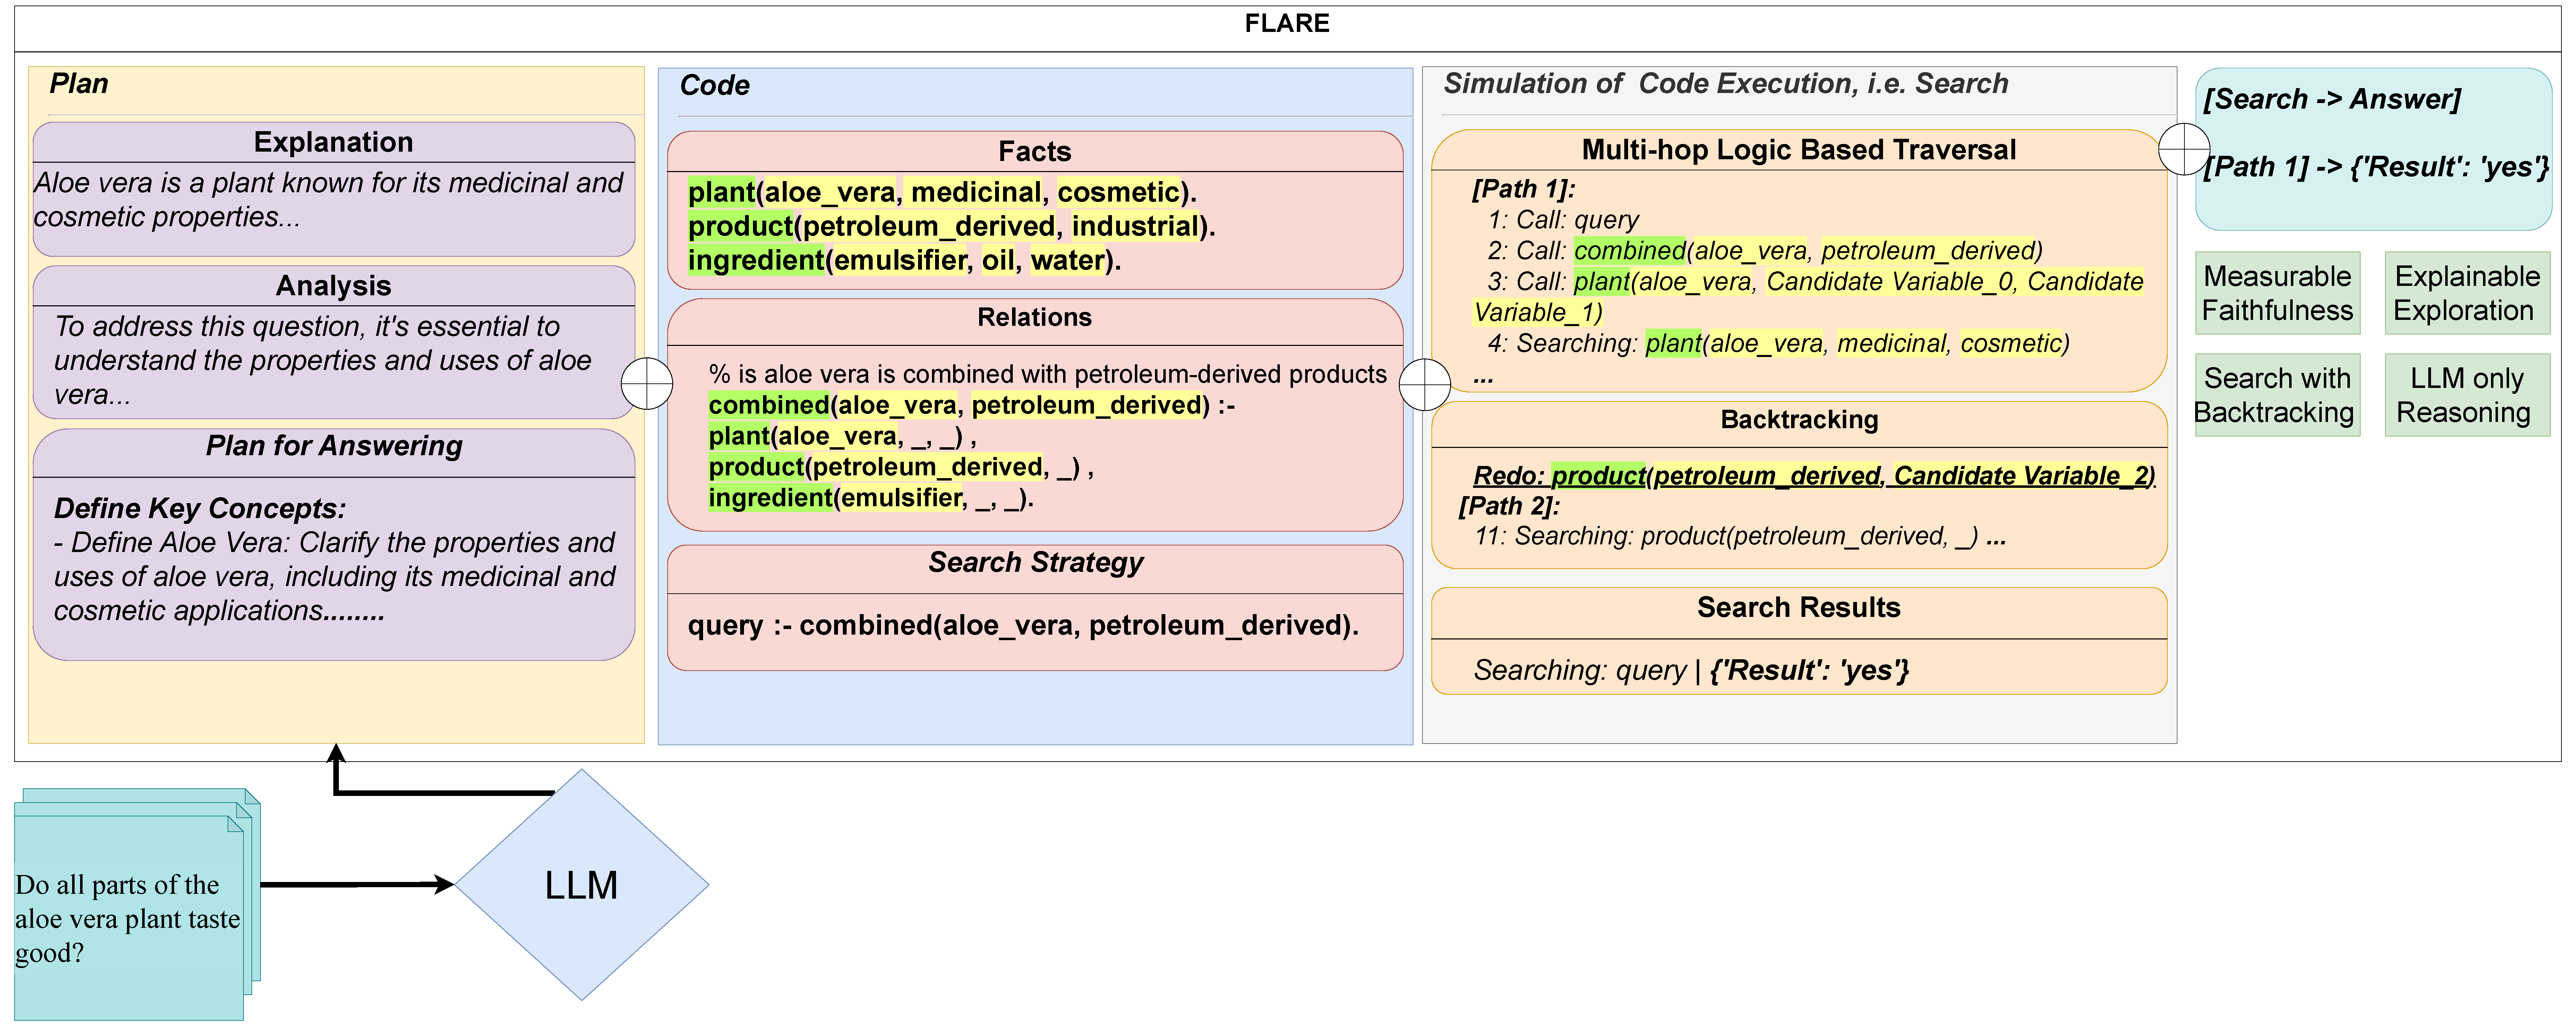
\includegraphics[width=\textwidth, clip]{figures/FLARE_splash_bare.pdf}
    \caption{A depiction of the \emph{plan}, \emph{code} and simulated \emph{search} in {\ours}. Each module has a breakdown of the relevant components composed by the LLM explained in \cref{sec:method}.}
    \label{fig:flare}
\end{figure*}
%
%
% \begin{figure}[t!]
%     \centering
%     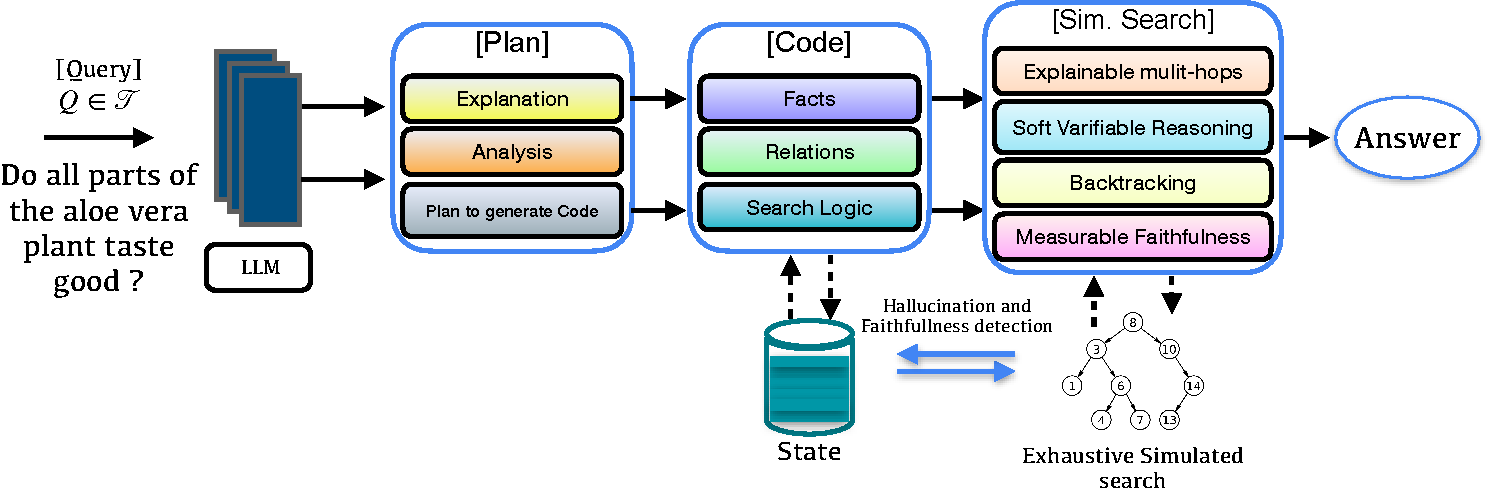
\includegraphics[width=\textwidth, clip]{figures/splash_alt-cropped.pdf}
%     % \caption{A direct comparison of CoT \cite{wei2022chain}, F-CoT \cite{DBLP:conf/acl/Xu0P0LH24} and \ours.}
%     \caption{An overview of the \emph{plan}, \emph{code} and \emph{search} modules used in \ours.}
%     \label{fig:flare}
% \end{figure}
%
To circumvent the problem of CoT faithfulness and allow for more robust reasoning during QA, \citet[Faithful CoT]{DBLP:conf/acl/Xu0P0LH24} suggested generating code which is further executed using an external symbolic solver.
%
Producing and executing code allows one to both create an output that can be conditioned on heuristic search in the problem space and perform backtracking.
%
However, strict translations of natural language queries into code, such as autoformalisation \citep{DBLP:conf/mkm/Szegedy20,DBLP:conf/mkm/WangKU18}, is a non-trivial task involving direct inference of implicit commonsense and domain-specific knowledge and the ability to align abstract and informal concepts directly to constrained formal definitions for further execution~\citep{DBLP:conf/nips/WuJLRSJS22}.
%
An example query \emph{``Do all parts of the aloe vera plant taste good?''} seen in \cref{fig:flare} is not trivial to formalise, nor to provide a strict algorithmic solution for it, making it much more suitable for soft reasoning.
%
Using external solvers makes such fuzzy reasoning impossible and requires consistently generating syntactically correct executable code.
%
While some LLMs have coding capabilities stemming from their pretraining \citep{DBLP:journals/corr/abs-2406-00515,DBLP:journals/corr/abs-2408-10914}, relative code consistency is more probable with models explicitly trained for coding \citep{DBLP:journals/corr/abs-2107-03374}.
%

%
To overcome these problems with CoT and F-CoT, we propose Faithful Logic-Aided Reasoning and Exploration (\ours), an interpretable method that allows for planning, fuzzy reasoning, and traversing the problem space with backtracking, exact task decomposition, and measuring faithfulness.
%
In \ours, given a natural language query, we prompt an LLM to sequentially generate a \emph{plan} that includes an analysis and the logical steps necessary for formalising and answering the question, a logical programming Prolog \citep{wielemaker2012swi} \emph{code} that allows formalising the query into a set of facts, relations and their composition forming the problem space and the \emph{search} which is an LLM generated simulation of exhaustive multi-hop traversal of that space from the code.
%
An illustration of {\ours} can be seen in \cref{fig:flare}.
%
In our framework, the generated code must not be consistently executable by an external solver, allowing for the soft-formalisation of natural language. Although we see that even generalist LLMs are able to produce executable code in $\geq 50\%$ of cases.
%
{\ours} allows us to measure the faithfulness of the outcome w.r.t. the simulated multi-hop logical traversal by directly comparing the search paths generated from executable Prolog code to that LLM generation. This comparison also allows for pinpointing model hallucinations and inconsistencies.
%
We systematically study the effectiveness of our method using $4$ general-purpose LLMs of varying scales across $9$ diverse benchmarks, covering Math World Problems, Multi-hop QA and Relation inference and show that our method achieves state-of-the-art results in $7$ out of $9$ in comparison to CoT and F-CoT. We also show that the method is rather competitive for models tuned for coding, with an average overall increase of $16\%$ over F-Cot and $9\%$ over CoT. Our findings show that model accuracy strongly correlates with the faithfulness of the reasoning process towards the problem space. We also provide ablations showing that the model can interpretably pinpoint hallucinations, search degeneracies, and the limitations of the search over the problem space. 
%
Our key contributions are the following: 
\begin{itemize}[leftmargin=*]
    \item We introduce {\ours} a novel paradigm for logic-aided and interpretable formalisation and search over the problem space in QA and reasoning tasks.
    \item We perform a systematic evaluation across $9$ benchmarks and $4$ models of varying scales, showing the advantages of using {\ours} for QA in a few-shot setup over prior approaches.
    \item The modularity of {\ours} allows defining a simple ingrained method for measuring model faithfulness and shows that it is strongly correlated with performance.
    \item We further show that using {\ours} allows us to interpretably and rigorously detect hallucinations along with sub-optimal and inconsistent reasoning patterns.
\end{itemize}

\section{Faithful Logic-Aided Reasoning and Exploration}
\label{sec:method}
\subsection{LLM Simulated Search}
\label{subsec:generate}

{\ours} comprises three modules for generating a \emph{plan}, \emph{code} and simulated \emph{search} for answering a natural language query $\mathcal{Q} = \{T_1 \dots T_{|\mathcal{Q}|}\}$, where each $T_i$ is a token.

\paragraph{Generating A Plan}
% 
For each query $\mathcal{Q}$, given an LLM $\mathcal{M}$, we initially prompt it to generate a \emph{plan}, $\mathcal{P}$, which should be comprised of task explanation, analysis and a plan for further formalising the query. An example of this can be seen in the \emph{plan} section in \cref{fig:flare}. We use in-context few shot examples $\mathcal{E}_{\mathcal{P}}$ of such \emph{plan} generations along with \textbf{greedy} decoding for obtaining the final plan.
%
\begin{align}
    \mathcal{P}_i \sim \argmax p_\mathcal{M}(T_i \mid \mathcal{E}_{\mathcal{P}}, \mathcal{Q})
\end{align}

\paragraph{Generating Code}

After generating the \emph{plan}, we prompt the LLM $\mathcal{M}$ to generate a Prolog code $\mathcal{C}$, an example of which can be seen in \cref{fig:flare}. We append executable code generation samples $\mathcal{C}_{\text{sample}}$ to the previous in-context examples $\mathcal{E}_{\mathcal{P}}$ and obtain few-shot code generation demonstrations $\mathcal{E}_{\mathcal{C}} =[\mathcal{E}_{\mathcal{P}};\mathcal{C}_{\text{sample}}]$
%
\begin{gather}
\label{eq:code}
     \mathcal{C}_i \sim \argmax p_\mathcal{M}(T_i \mid \mathcal{E}_{\mathcal{C}}, \mathcal{Q}, \mathcal{P})
     \\
     \mathcal{F}_{\text{\emph{code}}}, \mathcal{R}_{\text{\emph{code}}} , \mathcal{G}_{\text{\emph{code}}} = \text{EXTRACT}(\mathcal{C}_i) \nonumber
 \end{gather}

\paragraph{Benefits of Prolog}

Prolog is a symbolic logic-programming engine \citep{DBLP:conf/acm/Bowen79} used for heuristic search over Horn Clauses \citep{DBLP:journals/jlp/ChandraH85}. It is a declarative programming paradigm \citep{DBLP:conf/agp/Lloyd94}, meaning that the code is expressed as the logic of computation. In particular, this logic is formalised as a set of facts $\mathcal{F}$ and relations $\mathcal{R}$ forming our problem space, while the final goal $\mathcal{G}$ is a first-order logic combination of them. As a default, Prolog uses a depth-first search (DFS) strategy \citep{DBLP:conf/acm/Bowen79} for sub-goal decomposition and feasible traversal of the problem space that satisfies the goal $\mathcal{G}$. Such a traversal is referred to as the \emph{trace}. At each trace step, the program can either confirm or invalidate the sub-goal using the feasibility of fact and relation combinations, expand the search tree or retry satisfying a failed sub-goal with new combinations. An example of such a search can be observed in \cref{fig:flare}.
%
It is possible to complete an exhaustive search, exploring all possible paths that do or do not satisfy the goal. 
%
These characteristics are beneficial as we can explicitly access and segment the facts and relations that form the problem space and the search strategy used for query formalisation. As Prolog is declarative, it is sufficient to use a regexp heuristic for the segmentation, which is referred to as EXTRACT in \cref{eq:code} and \cref{eq:search}.
%
Furthermore, including exhaustive traversal traces in-context allows the LLM to simulate sub-goal decomposition, backtracking, intermediate goal invalidation, etc. We discuss this in more depth in the next paragraph.

\paragraph{Simulating Search}

After generating the logic-programming \emph{code}, we want to simulate program execution by generating a problem space traversal trace with our LLM $\mathcal{M}$. We update our in-context samples by appending search traces $\mathcal{S}_{\text{sample}}$ constructed from Prolog execution of sample codes $\mathcal{C}_{\text{sample}}$, i.e. $\mathcal{E}_{\mathcal{S}} =[\mathcal{E}_{\mathcal{C}};\mathcal{S}_{\text{sample}}]$. 
%
\begin{gather}
\label{eq:search}
     \mathcal{S}_i \sim \argmax p_\mathcal{M}(T_i \mid \mathcal{E}_{\mathcal{S}}, \mathcal{Q}, \mathcal{P}, \mathcal{C}) \\
     \mathcal{A}_{\text{\emph{search}}},
     \mathcal{F}_{\text{\emph{search}}}, \mathcal{R}_{\text{\emph{search}}} = \text{EXTRACT}(\mathcal{S}_i) \nonumber
 \end{gather}
%
 During iterative problem space traversal, we can segment the facts $\mathcal{F}_{\text{\emph{search}}}$, relations $\mathcal{R}_{\text{\emph{search}}}$, completed and backtracked paths with their answers $\mathcal{A}_{\text{\emph{search}}}$ used during the search simulation. To get the final answer we update in-context samples with the correct final answers $\mathcal{A}_{\text{sample}}$ from the executed search $\mathcal{S}_{\text{sample}}$, $\mathcal{E}_{\mathcal{A}} =[\mathcal{E}_{\mathcal{S}};\mathcal{A}_{\text{sample}}]$. 
%
 \begin{align}
      \mathcal{A}_{\text{\emph{Final}}} \sim \argmax p_\mathcal{M}(T_i \mid \mathcal{E}_{\mathcal{A}}, \mathcal{Q}, \mathcal{P}, \mathcal{C}, \mathcal{})
 \end{align}
%
The prompts used for generating each part in {\ours} can be seen in \cref{append:prompts}. 

\subsection{Detecting Reasoning Inconsistencies}
\label{subsec:reasoning_inc}

For each query $\mathcal{Q}$ given the \emph{code} $\mathcal{C}$ and the simulated \emph{search} $\mathcal{S}$ along with the extracted facts $\mathcal{F}_{\text{\emph{code}}}, \mathcal{F}_{\text{\emph{search}}}$ and relations $\mathcal{R}_{\text{\emph{code}}}, \mathcal{R}_{\text{\emph{search}}}$ from each designated module, we aim to detect the inconsistencies during the reasoning process of the LLM. We use exact string matching between all these facts and relations in \emph{code} and simulated \emph{search}.
%
\begin{gather}
% \mathds{1}: \mathcal{F}_{\text{\emph{code}}} \times \mathcal{F}_{\text{\emph{search}}} \times \mathcal{R}_{\text{\emph{code}}} \times \mathcal{R}_{\text{\emph{search}}} \rightarrow \{0, 1\} = \begin{cases}
%       1 \quad \text{if} \quad \mathcal{F}^{i_{\text{match}}}_{\text{\emph{code}}} = \mathcal{F}^{j_{\text{match}}}_{\text{\emph{search}}} \{\forall i, j: \exists i_{\text{match}}, j_{\text{match}} \} \\
%        \mathcal{R}^i_{\text{\emph{code}}} = \mathcal{R}^j_{\text{\emph{search}}} \exists i, j
% \end{cases}
\forall i, \exists j \quad \text{such that} \quad \mathcal{F}_{\text{code}}^i = \mathcal{F}_{\text{search}}^j \quad \text{and} \quad \forall v, \exists q \quad \mathcal{R}_{\text{code}}^v = \mathcal{R}_{\text{search}}^q \\
\forall j, \exists i \quad \text{such that} \quad \mathcal{F}_{\text{code}}^i = \mathcal{F}_{\text{search}}^j \quad \text{and} \quad \forall q, \exists v \quad \mathcal{R}_{\text{code}}^v = \mathcal{R}_{\text{search}}^q
\end{gather}
%
With this framework in mind, we define two reasoning failure modes. 
%
In the \emph{first} failure mode, given that some fact or relation was used in the simulated \emph{search} but did not exist in the generated \emph{code}, i.e. $\exists j \text{ such that } \mathcal{F}_{\text{search}}^j \notin \mathcal{F}_{\text{code}}$, we claim that the LLM has \emph{hallucinated}. We postulate that the model either produced incomplete knowledge during formalisation to \emph{code} or created a piece of non-existing information during the \emph{search}. We do not consider facts that emerged during a direct inference step within the simulated search during our calculation. For example, if we are dealing with a mathematical query $4\cdot (5+6) = ?$, the search would involve separately evaluating the expression $5+6=11$. In this case, $11$ will not be treated as a hallucinated fact within the search but rather as an emergent fact obtained from direct inference.   
%
The \emph{second} failure mode is the reciprocal case, where a fact or relation present in the \emph{code} is not used during the \emph{search}. We refer to this phenomenon as \emph{sub-optimal reasoning} as it shows that the LLM could not explore the problem space completely or injected unsuitable knowledge during formalisation into \emph{code}. 

\section{Empirical Evaluation}
We trained a series of models of various sizes. For all subsequent evaluations, we will use the largest model (referred to as CogVideoX).
In this section, we present the experimental validation of CogVideoX through two primary methods: automated metric evaluation and human assessment, providing a thorough analysis of the performance and quality of the generated videos. 
We trained a series of models with different parameter sizes. The following evaluation defaults to using our largest model.

\subsection{Results of Automated Metric Evaluation} 

\paragraph{Baselines.} We chose several top-performing text-to-video models as our baselines for comparison, including T2V-Turbo~\citep{li2024t2v}, AnimateDiff~\citep{guo2023animatediff}, VideoCrafter2~\citep{chen2024videocrafter2}, OpenSora~\citep{opensora}, Show-1~\citep{zhang2023show}, Gen-2~\citep{gen2}, Pika~\citep{pika} and LaVie-2~\citep{wang2023lavie}.


% \begin{figure}[h]
% \begin{center}
% \includegraphics[width=0.9\linewidth]{images/bench_eval.png}
% \end{center}
% \caption{The radar chart comparing the performance of different models.}
% \label{fig:radar}
% \end{figure}

\hide{
%\begin{wrapfigure}{r}{0.5\textwidth}
\begin{figure}
\centering
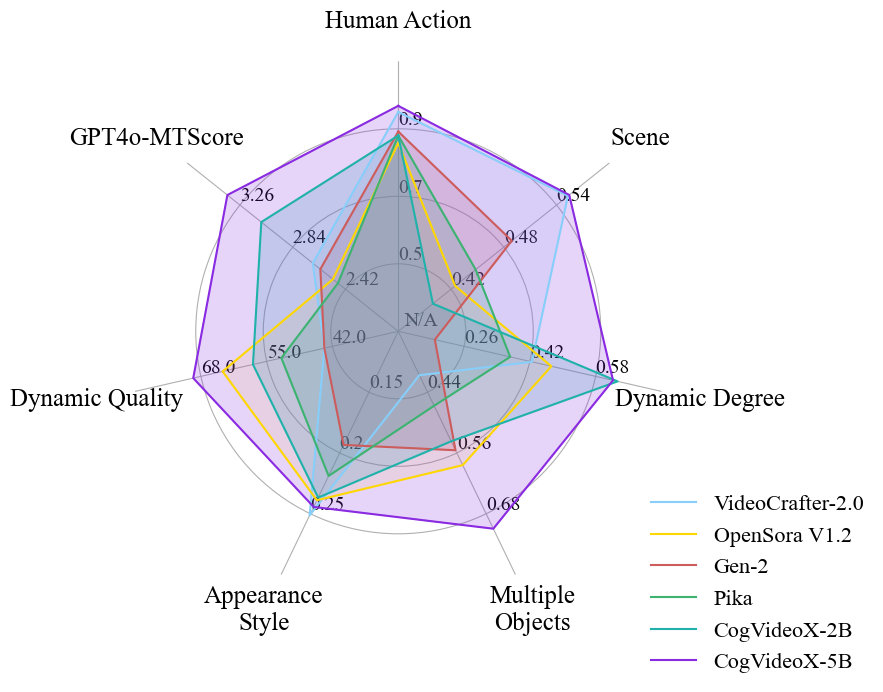
\includegraphics[width=0.7\linewidth]{images/bench_eval9.png}
\caption{The radar chart comparing the performance of different models. CogVideoX represents the largest one. It is clear that CogVideoX outperforms its competitors in the vast majority of metrics, and it is very close to the leading models in the remaining indicator.
}
\label{fig:radar}
% \vspace{-10mm}
%\end{wrapfigure}

\end{figure}

}%end ofhide
\paragraph{Evaluation Metrics.} To evaluate the text-to-video generation, we employed several metrics from VBench~\citep{huang2023vbench}: \emph{Human Action}, \emph{Scene}, \emph{Dynamic Degree}, \emph{Multiple Objects}, and \emph{Appearance Style}. VBench is a suite of tools designed to automatically assess the quality of generated videos. We have selected certain metrics from VBench, excluding others that do not align with our evaluation needs. For example, the color metric, intended to measure the presence of objects corresponding to specific colors across frames in the generated video, assesses the model's quality by calculating the probability. However, this metric may mislead video generation models that exhibit greater variation, thus we chose not to include it in our evaluation. For longer-generated videos, some models might produce videos with minimal changes between frames to obtain higher scores, but these videos lack rich content. Therefore, a metric for evaluating the dynamism of the video becomes more important. To address this, we employed two video evaluation tools, We also employed the \emph{Dynamic Quality} from Devil~\citep{liao2024evaluationtexttovideogenerationmodels} and \emph{GPT4o-MTScore} from ChronoMagic~\citep{yuan2024chronomagic}, which focus more on the dynamic characteristics of videos. \emph{Dynamic Quality} is defined by the integration of various quality metrics with dynamic scores. This approach mitigates biases arising from negative correlations between video dynamics and video quality, leading to a more thorough assessment of video quality. ChronoMagic, for instance, introduces the \emph{GPT4o-MTScore}, a metric designed to measure the metamorphic amplitude of time-lapse videos, such as those depicting physical, biological, and meteorological changes. This metric is obtained by extracting frames from the generated videos at regular intervals and using GPT-4o~\citep{gpt4o} to score the degree of change, providing a fine-grained assessment of video dynamism. This method ensures a more accurate evaluation of the content's variability over time, countering the potential bias of static frame sequences in scoring.



\paragraph{Results.} Table~\ref{table:results} provides a detailed comparison of the performance of our CogVideoX model with other models. Our model achieved the best performance in 5 out of the 7 metrics and showed competitive results in the remaining 2 metrics. These results demonstrate that our model not only excels in video generation quality but also outperforms previous models in handling various complex dynamic scenes. Additionally, Figure~\ref{fig:radar} presents a radar chart comparing the performance of different models.


\begin{figure}[ht]
\begin{center}
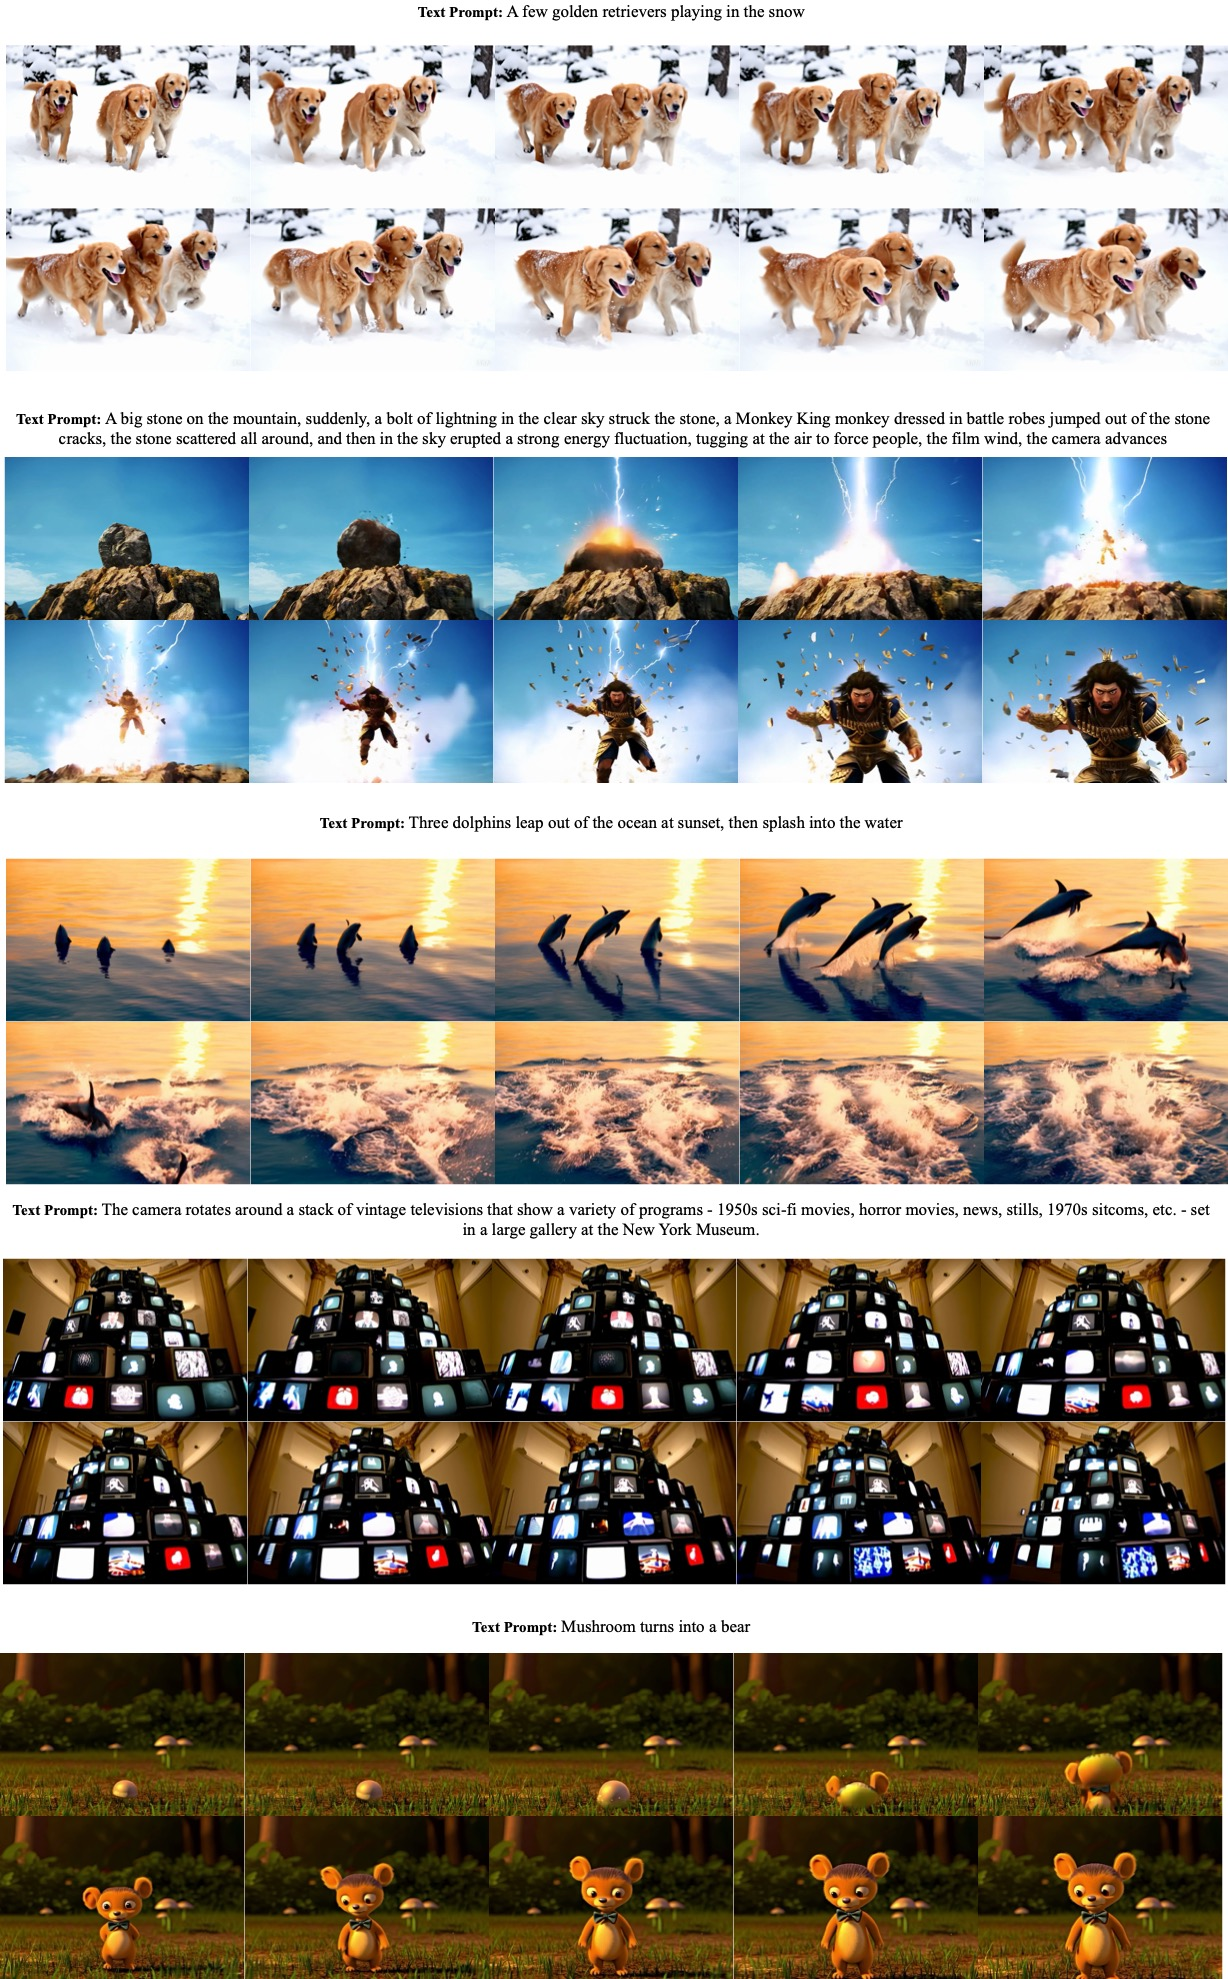
\includegraphics[width=\linewidth]{images/t2v/goodcase1.jpg}
\end{center}
\caption{Text to video showcases. The displayed prompt will be upsampled before being fed into the model. The generated videos contain large motion and can produce various video styles.}
\label{fig:t2vgood1}
\end{figure}

\begin{figure}[ht]
\begin{center}
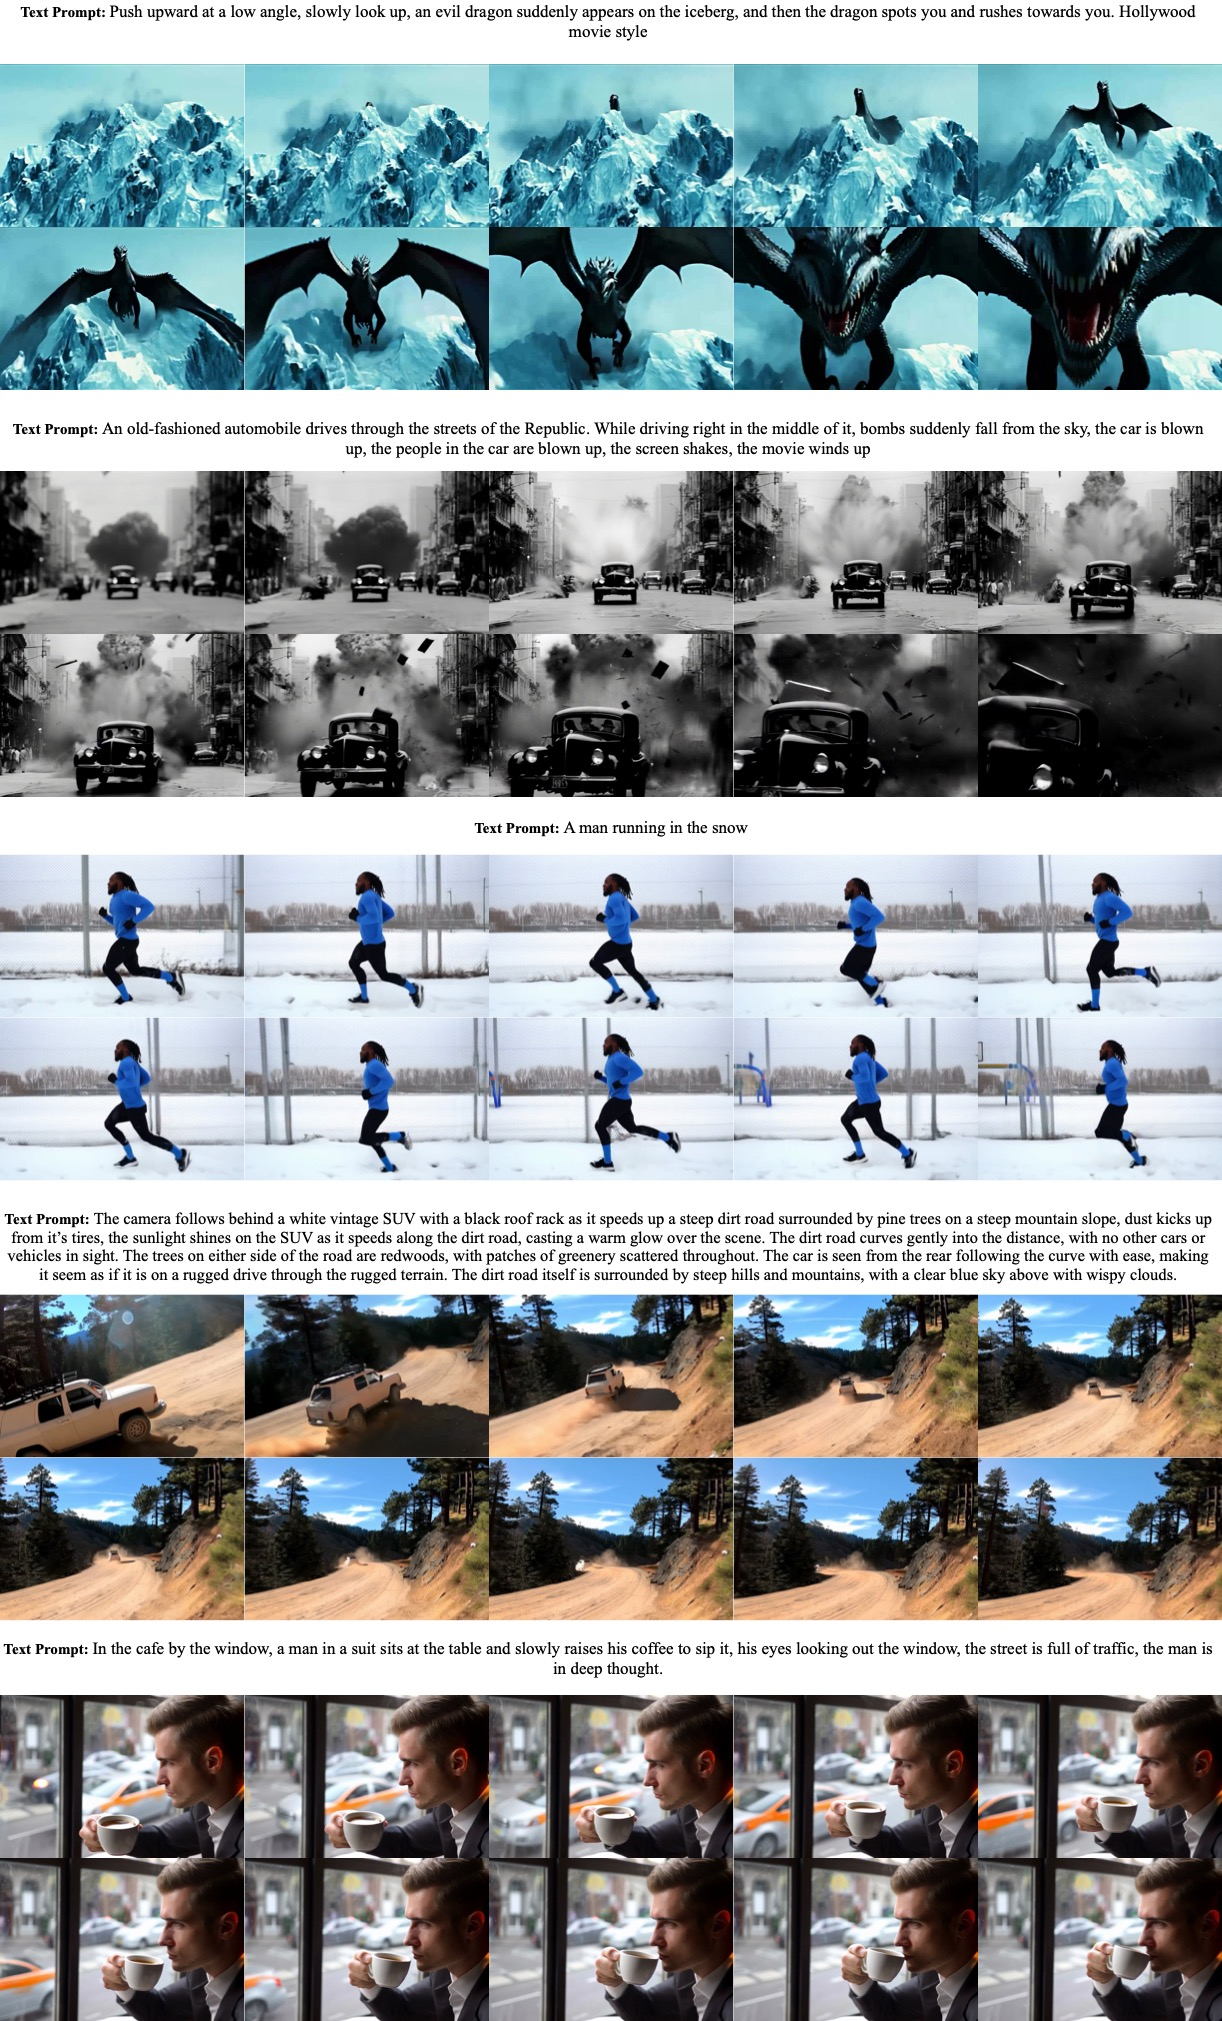
\includegraphics[width=0.98\linewidth]{images/t2v/goodcase2.jpg}
\end{center}
\caption{Text to video showcases.}
\label{fig:t2vgood2}
\end{figure}


% Please add the following required packages to your document preamble:
% \usepackage[table,xcdraw]{xcolor}
% Beamer presentation requires \usepackage{colortbl} instead of \usepackage[table,xcdraw]{xcolor}
% \usepackage[normalem]{ulem}
% \useunder{\uline}{\ul}{}




% \begin{table}[]

% \centering
% \setlength\tabcolsep{3pt}

% \label{sample-table}
% \small
% \vspace{-10pt}
% \caption{\textbf{Automatic Evaluation Results per Dimension.}The table presents a comparative analysis of various video models across different dimensions. It is evident from the table that, in terms of both human motion and background effects as well as the accuracy and distinctiveness of objects, CogVideoX has achieved the current SOTA level. Furthermore, CogVideoX has garnered a commendable score in the expression of dynamic qualities, a capability that serves as a more precise indicator of the intrinsic properties of video media, distinct from the static nature of photographic images.}

% \vspace{6pt}

% \begin{tabular}{cccccccc}
% \toprule
% \multirow{2}{*}{\textbf{Models} }  & \textbf{human}  & \textbf{object} &\multirow{2}{*}{\textbf{scene}}&\textbf{dynamic} &\textbf{multiple} &\textbf{spatial} &\textbf{appearance} \\
%     & \textbf{action}& \textbf{class}& & \textbf{degree} &\textbf{objects}& \textbf{relationship}&\textbf{style}  
% \\
% \midrule
% CogVideoX & 96.80\% &93.70\% & 55.44\% & 62.22\% & 70.95\% & 61.29\% & 24.44\% \\
% {LaVie-2} & 96.40\% & 97.52\%  & 49.59\% & 31.11\% & 64.88\%  & 38.68\% & 25.09\%  \\
% {T2V-Turbo}  & 95.20\%  & 93.96\%& 55.58\% & 49.17\% & 54.65\%    & 38.67\%  & 24.42\%   \\
% {Gen-2}  & 89.20\%& 90.92\%  & 48.91\%  & 18.89\% & 55.47\%    & 66.91\%   & 19.34\%  \\
% {VideoCrafter-2.0\citep{chen2024videocrafter2}} & 95.00\% & 92.55\% & 55.29\%               & 42.50\% & 40.66\% & 35.86\% & 25.13\%  \\
% {Pika Beta} & 88.00\% & 87.45\%  & 44.80\% & 37.22\% & 46.69\% & 65.65\% & 21.89\%   \\
% AnimateDiff-V2 & 92.60\% & 90.90\%  & 50.19\% & 40.83\%        & 36.88\% & 34.60\%  & 22.42\%\\
% {OpenSora V1.2}   & 85.80\% & 83.37\%& 42.47\%   & 47.22\%    & 58.41\% & 67.51\%  & 23.89\%  \\
% {Show-1} & 95.60\%  & 93.07\%  & 47.03\% & 44.44\% & 45.47\% & 53.50\%  & 23.06\%  \\
% {HiGen}  & 86.20\%  & 86.06\%  & 44.88\% & 99.17\% & 22.39\%  & 22.43\% & 24.54\% \\  
% \bottomrule
% \end{tabular}
% \end{table}



% \iffalse



% \begin{table}[ht!]
% \centering
% \caption{Evaluation results.}
% \setlength\tabcolsep{3pt}
% \label{sample-table}
% \begin{center}
% \small
% \resizebox{0.9\linewidth}{!}{
% \begin{tabular}{ccccccccc}

% \multirow{2}{*}{\textbf{Models} }  & \textbf{subject}  & \textbf{background} &\textbf{temporal} &\textbf{motion} &\textbf{dynamic} &\textbf{aesthetic} &\textbf{imaging} &\textbf{object} \\
%     & \textbf{consistency}& \textbf{consistency}& \textbf{flickering}& \textbf{smoothness} &\textbf{degree}& \textbf{quality}&\textbf{quality} & \textbf{class}
% \\ \hline 
%         CogVideoX & 94.66\% & 95.92\% & 97.47\% & 98.10\% & 62.22\% & 55.14\% & 63.62\% & 93.70\%  \\
%         LaVie-2 & 97.90\% & 98.45\% & 98.76\% & 98.42\% & 31.11\% & 67.62\% & 70.39\% & 97.52\%  \\ 
%         T2V-Turbo (VC2) & 96.28\% & 97.02\% & 97.48\% & 97.34\% & 49.17\% & 63.04\% & 72.49\% & 93.96\%  \\ 
%         Gen-2 (2023-06) & 97.61\% & 97.61\% & 99.56\% & 99.58\% & 18.89\% & 66.96\% & 67.42\% & 90.92\%  \\ 
%         VideoCrafter-2.0\citep{chen2024videocrafter2} & 96.85\% & 98.22\% & 98.41\% & 97.73\% & 42.50\% & 63.13\% & 67.22\% & 92.55\%  \\ 
%         Pika Beta (2023-06) & 96.76\% & 98.95\% & 99.77\% & 99.51\% & 37.22\% & 63.15\% & 62.33\% & 87.45\%  \\ 
%         AnimateDiff-V2 & 95.30\% & 97.68\% & 98.75\% & 97.76\% & 40.83\% & 67.16\% & 70.10\% & 90.90\%  \\ 
%         OpenSora V1.2 & 94.45\% & 97.90\% & 99.47\% & 98.20\% & 47.22\% & 56.18\% & 60.94\% & 83.37\%  \\ 
%         Show-1 & 95.53\% & 98.02\% & 99.12\% & 98.24\% & 44.44\% & 57.35\% & 58.66\% & 93.07\%  \\ 
%         HiGen & 90.07\% & 93.99\% & 93.24\% & 96.69\% & 99.17\% & 57.30\% & 63.92\% & 86.06\% \\ 
% \hline \\

% \multirow{2}{*}{\textbf{Models} }  & \textbf{multiple}  & \textbf{human} &\multirow{2}{*}{\textbf{color}} &\textbf{spatial} &\multirow{2}{*}{\textbf{scene}} &\textbf{appearance} &\textbf{temporal} &\textbf{overall} \\
%     & \textbf{objects}& \textbf{action}& & \textbf{relation} & & \textbf{style}&\textbf{style} & \textbf{consistency}
% \\ \hline 
%         CogVideoX & 70.95\% & 96.80\% & 79.75\% & 61.29\% & 55.44\% & 24.44\% & 23.69\% & 26.73\%  \\ 
%         LaVie-2 & 64.88\% & 96.40\% & 91.65\% & 38.68\% & 49.59\% & 25.09\% & 25.24\% & 27.39\%  \\ 
%         T2V-Turbo (VC2) & 54.65\% & 95.20\% & 89.90\% & 38.67\% & 55.58\% & 24.42\% & 25.51\% & 28.16\%  \\
%         Gen-2 (2023-06) & 55.47\% & 89.20\% & 89.49\% & 66.91\% & 48.91\% & 19.34\% & 24.12\% & 26.17\%  \\ 
%         VideoCrafter-2.0 & 40.66\% & 95.00\% & 92.92\% & 35.86\% & 55.29\% & 25.13\% & 25.84\% & 28.23\%  \\
%         Pika Beta (2023-06) & 46.69\% & 88.00\% & 85.31\% & 65.65\% & 44.80\% & 21.89\% & 24.44\% & 25.47\%  \\ 
%         AnimateDiff-V2 & 36.88\% & 92.60\% & 87.47\% & 34.60\% & 50.19\% & 22.42\% & 26.03\% & 27.04\%  \\ 
%         OpenSora V1.2 & 58.41\% & 85.80\% & 87.49\% & 67.51\% & 42.47\% & 23.89\% & 24.55\% & 27.07\%  \\ 
%         Show-1 & 45.47\% & 95.60\% & 86.35\% & 53.50\% & 47.03\% & 23.06\% & 25.28\% & 27.46\%  \\ 
%         HiGen & 22.39\% & 86.20\% & 86.22\% & 22.43\% & 44.88\% & 24.54\% & 25.14\% & 27.14\% \\ \hline

% \hline \\
% \end{tabular}

% }
% \end{center}
% \end{table}

% \fi






% \begin{table}[!ht]
% \centering

% \label{sample-table}
% \small
% \vspace{-10pt}
% \caption{\textbf{Automatic Evaluation Results per Dimension.}}

% \vspace{6pt}

% \resizebox{0.8\linewidth}{!}{
%     \begin{tabular}{cccc}
%         \textbf{Models} & \textbf{\Centerstack{Dynamics Range}} & \textbf{\Centerstack{Dynamics Controllability}} & \textbf{\Centerstack{Dynamics-based Quality}} \\ \hline
%         CogVideoX       & 55.7 & 71.8 & \textbf{69.5} \\ 
%         Gen-2           & 30.8 & \textbf{82.5} & 43.6 \\ 
%         Pika            & 43.2 & 72.0 & 52.1 \\ 
%         VideoCrafter2   & 34.1 & 57.0 & 43.6 \\ 
%         OpenSora        & \textbf{61.2} & 62.4 & 63.7 \\ 
%         Show-1          & 45.1 & 73.9 & 57.7 \\ 
%     \end{tabular}
% }
% \end{table}


% \begin{figure}[h]
% \begin{center}
% \includegraphics[width=0.9\linewidth]{images/bench_eval.png}
% \end{center}
% \caption{The radar chart comparing the performance of different models.}
% \label{fig:radar}
% \end{figure}

\hide{
%\begin{wrapfigure}{r}{0.5\textwidth}
\begin{figure}
\centering
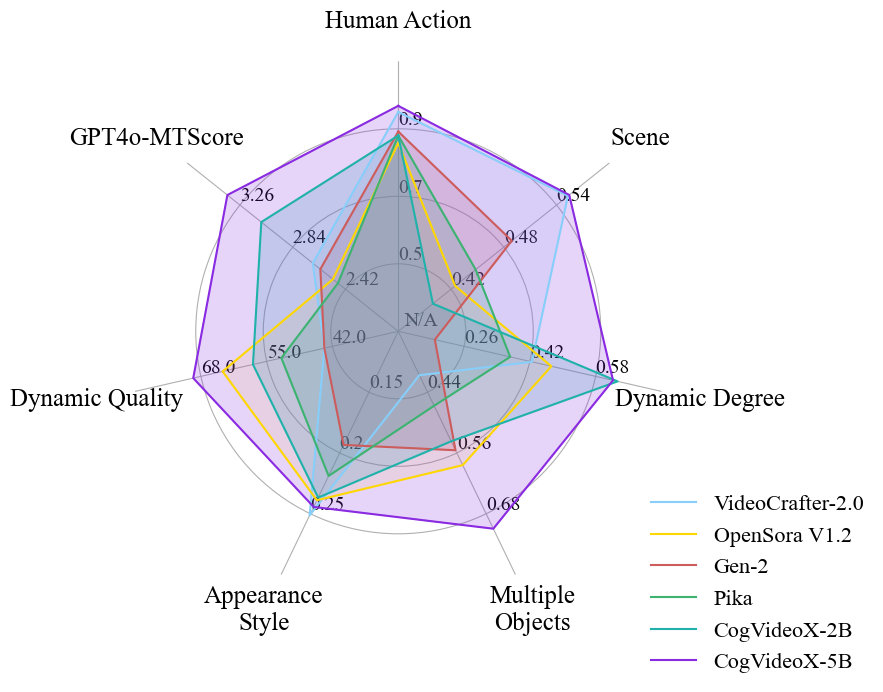
\includegraphics[width=0.7\linewidth]{images/bench_eval9.png}
\caption{The radar chart comparing the performance of different models. CogVideoX represents the largest one. It is clear that CogVideoX outperforms its competitors in the vast majority of metrics, and it is very close to the leading models in the remaining indicator.
}
\label{fig:radar}
% \vspace{-10mm}
%\end{wrapfigure}

\end{figure}

}%end ofhide


\subsection{Human Evaluation}
In addition to automated scoring mechanisms, a comparative analysis between the Kling~\citep{kling} and CogVideoX was conducted using a manual scoring system. One hundred meticulously crafted prompts were used, characterized by their broad distribution, clear articulation, and well-defined conceptual scope. We randomize videos for blind evalution. A panel of evaluators assigned scores for each detail on a scale from zero to one, with the overall total score rated on a scale from zero to five, where higher scores reflect better video quality. Reasons for any score deductions were also carefully documented. The results shown in Table~\ref{table:human_eva} indicate that our model outperforms Kling in all aspects. More details are shown in \ref{sec:human_evalution}.

\begin{table}[!ht]
\centering
\label{sample-table}
\small
\vspace{-5pt}
\caption{Human evaluation between CogVideoX and Kling.}
\label{table:human_eva}
\resizebox{0.75\linewidth}{!}{
    \begin{tabular}{cccccc}
    \toprule
        Model & \Centerstack{Sensory\\Quality} & \Centerstack{Instruction\\Following}&\Centerstack{Physics\\Simulation} & \Centerstack{Cover\\Quality} & 
        \Centerstack{Total\\Score} \\ 
        \midrule
        Kling & 0.638 & 0.367 & 0.561 & 0.668 & 2.17 \\
        \midrule
         {\bf CogVideoX-5B} & {\bf 0.722} & {\bf 0.495} & {\bf 0.667} & {\bf 0.712} & {\bf 2.74}  \\
        \bottomrule
    \end{tabular}
}
\vspace{-3mm}
\end{table}



% \begin{table}[!ht]
% \centering

% \label{sample-table}
% \small
% \vspace{-10pt}
% \caption{\textbf{Automatic Evaluation Results per Dimension.}}

% \vspace{6pt}

% \resizebox{0.8\linewidth}{!}{
%     \begin{tabular}{cccc}
%         \textbf{Models} & \textbf{\Centerstack{Dynamics Range}} & \textbf{\Centerstack{Dynamics Controllability}} & \textbf{\Centerstack{Dynamics-based Quality}} \\ \hline
%         CogVideoX       & 55.7 & 71.8 & \textbf{69.5} \\ 
%         Gen-2           & 30.8 & \textbf{82.5} & 43.6 \\ 
%         Pika            & 43.2 & 72.0 & 52.1 \\ 
%         VideoCrafter2   & 34.1 & 57.0 & 43.6 \\ 
%         OpenSora        & \textbf{61.2} & 62.4 & 63.7 \\ 
%         Show-1          & 45.1 & 73.9 & 57.7 \\ 
%     \end{tabular}
% }
% \end{table}


\subsection{Measuring Faithfulness}

We propose a method to measure the faithfulness of the LLM reasoning process when using {\ours}. As mentioned in \cref{subsec:generate}, for each query in a dataset $\mathcal{D} = [\mathcal{Q}_1, \dots ,\mathcal{Q}_{|\mathcal{D}|}]$, we generate a set of codes $\Phi = [\mathcal{C}_1, \dots ,\mathcal{C}_{|\Phi|}]$ and simulated problem space searches $\Psi = [\mathcal{S}_1, \dots, \mathcal{S}_{|\Psi|}]$. We use the Prolog engine to execute all of the codes $\Phi$ and obtain a set of correctly written programs $\Phi^\prime$ and exact search paths $\Psi^\prime$. As we do not require explicit programmatic correctness during inference in {\ours} for any code $\mathcal{C}_i$, some Prolog executions resulting in an error are filtered out in $\Psi^\prime$. To assess model reasoning faithfulness towards code formalisations, we compare the search paths $\Phi^\prime$ obtained from Prolog execution with their designated counterparts $\Phi_{\text{\emph{gen}}}^\prime$ generated by the LLM from the same code. We use ROUGE \citep{lin-2004-rouge} to compute the matching score for each executed and simulated search path. In particular, we use ROUGE-Lsum, which uses the longest common subsequence (LCS) over each line to obtain the final score. This method fits our cause as a line in a Prolog search execution represents a single logic step within the traversal. This allows us to measure the similarity of the reasoning contents and structure in exact and simulated searches.  

\section{Experimental Setup}
\label{sec:ex_setup}
\subsection{Datasets}
To evaluate {\ours}, we use a benchmark of $9$ tasks that cover Math Word Problems (MWP), multi-hop QA and relation inference. For testing numeric and mathematical reasoning, we follow CoT \citep{wei2022chain} by including GSM8K \citep{DBLP:journals/corr/abs-2110-14168}, SVAMP \citep{DBLP:conf/naacl/PatelBG21}, MultiArith \citep{DBLP:conf/emnlp/RoyR15}, ASDiv \citep{DBLP:conf/acl/MiaoLS20} and AQuA \citep{DBLP:conf/acl/LingYDB17}. Among these, GSM8K, SVAMP, MultiArith and ASDiv cover elementary and middle school arithmetic word problems with a set of integers or decimals as the answer. AQuA is a multiple-choice numerical, symbolic reasoning dataset where each answer is a mathematical expression containing notations, values and expressions not defined in the query.
%
We also test {\ours} using three multi-hop QA datasets. We use StrategyQA \citep{DBLP:journals/tacl/GevaKSKRB21}, which is a boolean QA task that requires sub-goal decomposition and a multi-hop reasoning strategy to answer. The example \emph{``Do all parts of the aloe vera plant taste good?''} used in \cref{fig:flare}, is taken from StratedyQA. The multi-hop QA testing also includes Date and Sports Understanding, subsets of BIG-Bench \citep{srivastava2023beyond}. The tasks involve inferring an exact date given some calculations in the relative time period and understanding if an artificially created sports statement is feasible.
%
Finally, we assess {\ours} on Relational Inference using CLUTRR \citep{DBLP:conf/emnlp/SinhaSDPH19}, which involves inferring the familial relation between two entities mentioned in a natural language description of the partial family graph. 
%
We adopt the same in-context samples used in \citep{DBLP:conf/acl/Xu0P0LH24, wei2022chain}. The complete descriptions, statistics and examples for each dataset can be found in \cref{tab:data_stat} in \cref{append:prompts}. 

\begin{figure}[t!]
    \centering
    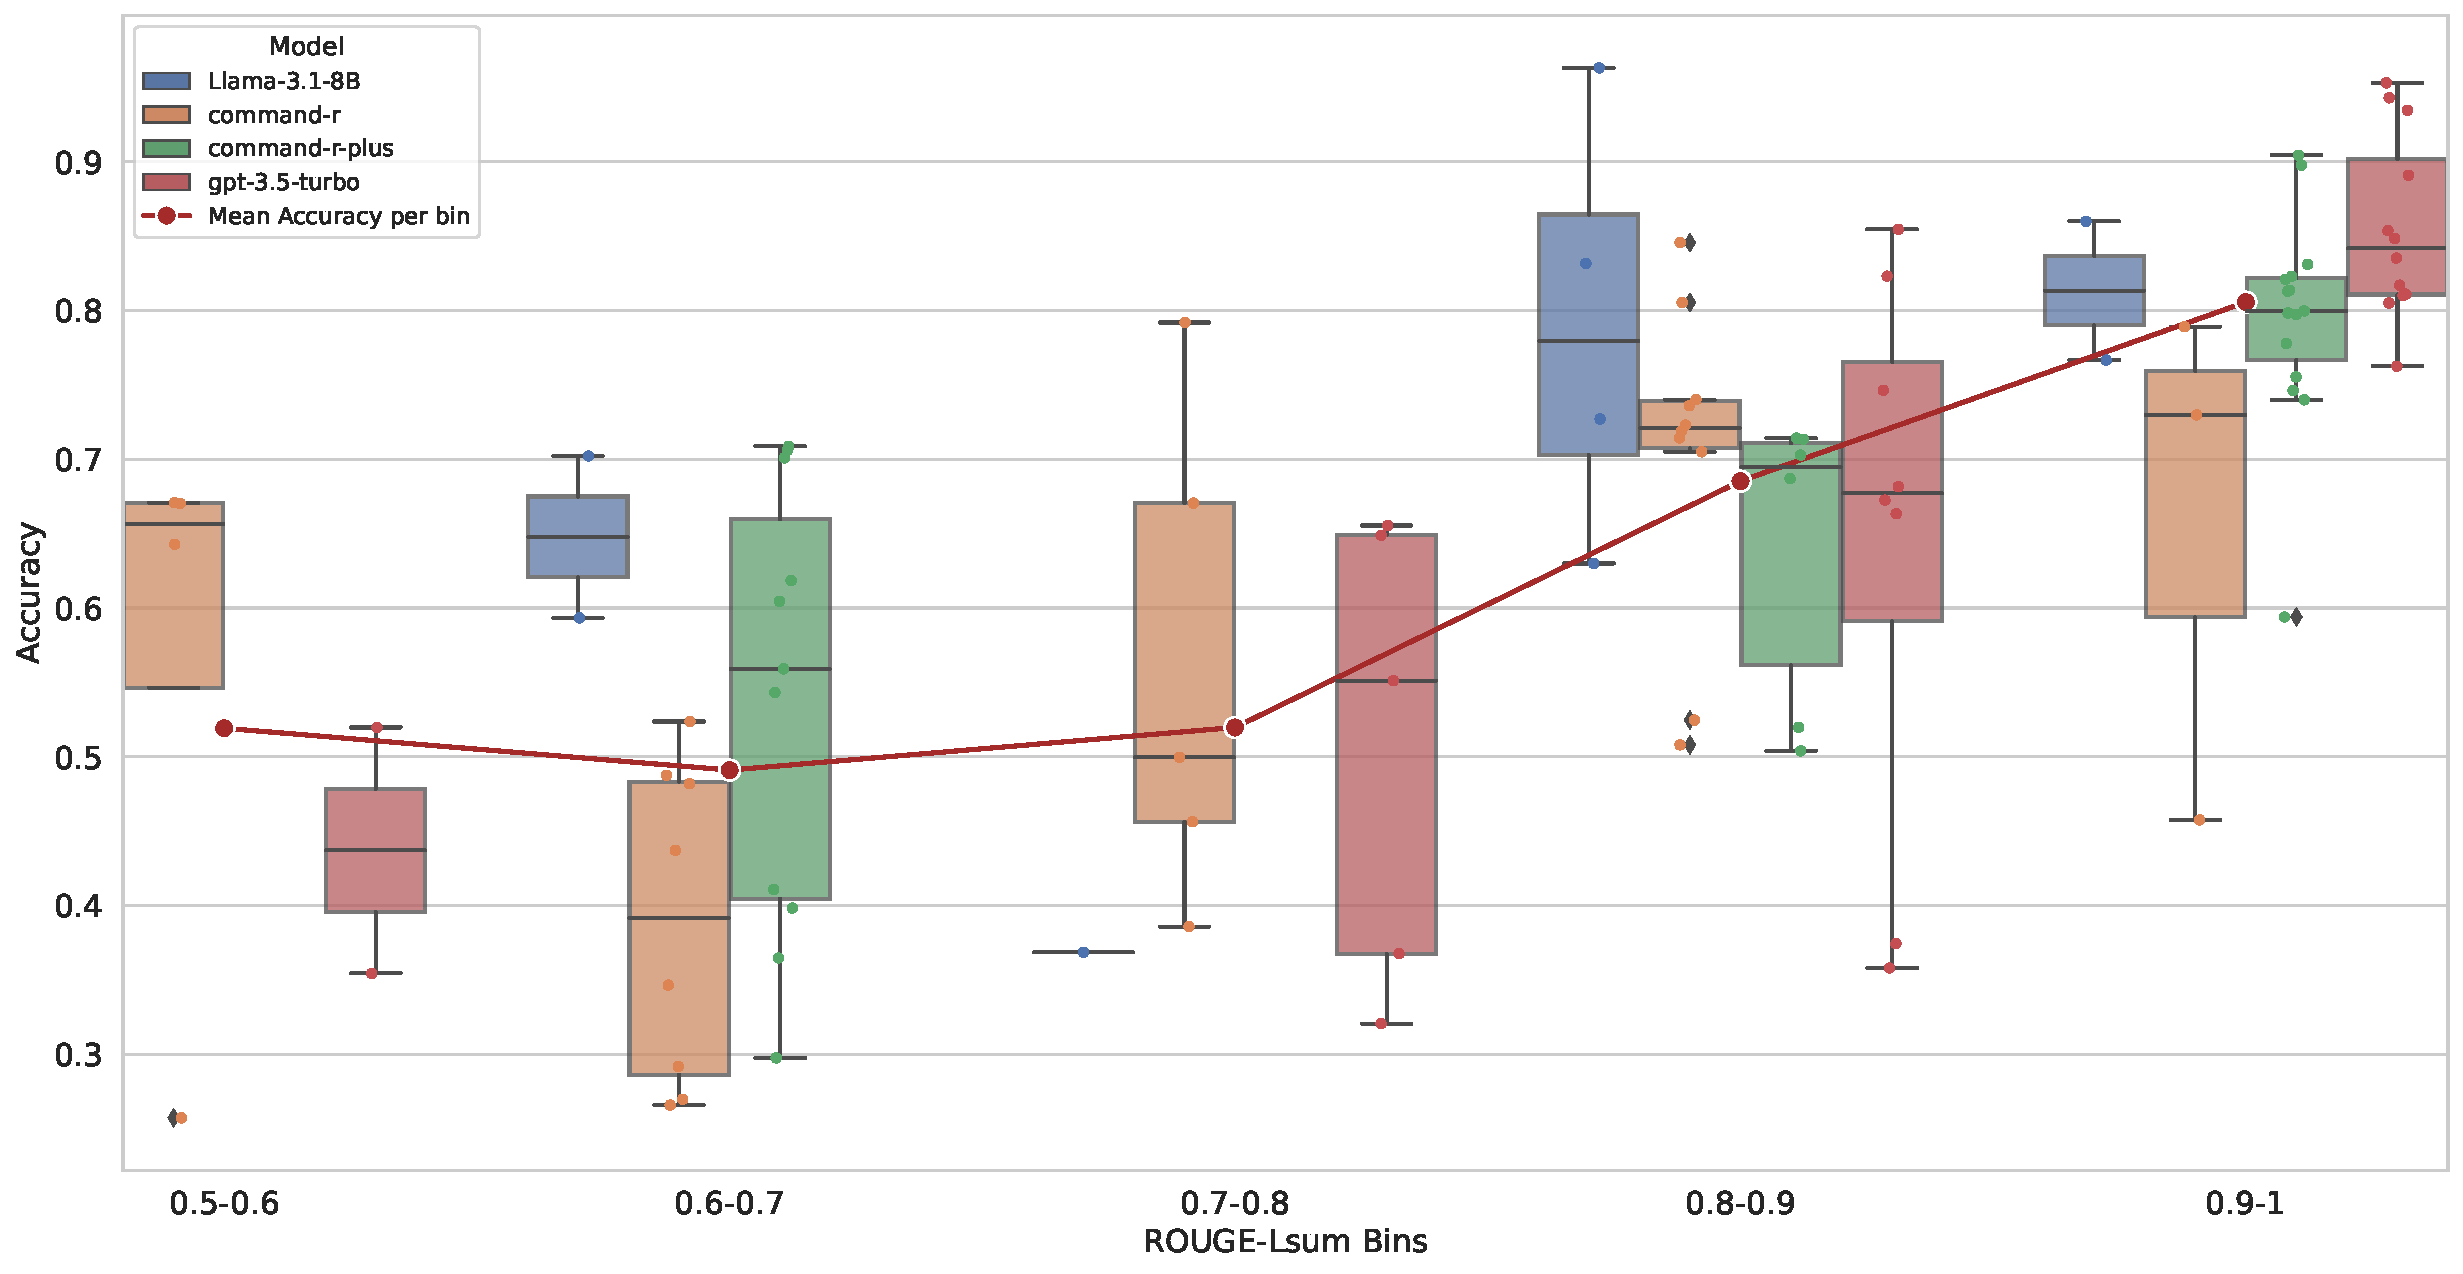
\includegraphics[clip=true,width=\textwidth]{figures/model_accuracy_vs_rouge_All_Datasets.pdf}
    \caption{The trend of mean model accuracy w.r.t mean faithfulness (ROUGE-Lsum) for all the models. Faithfulness is positively correlated with model performance.}
    \label{fig:faith_vs_acc}
\end{figure}

\subsection{Benchmarks}

We compare {\ours} with CoT \citep{wei2022chain} as a prompting method that reasons using natural language chains and with F-CoT \citep{DBLP:conf/acl/Xu0P0LH24} that formalises the query into a code and offload the reasoning to an external symbolic solver. We use Llama3.1 (8B) \citep{DBLP:journals/corr/abs-2407-21783}, CmDR (30B) \citep{cohere2024commandr}, CmDR+ (100B) \citep{cohere2024commandr}  and GPT3.5 \citep{DBLP:conf/nips/BrownMRSKDNSSAA20} ($\geq 100B$ \citep{DBLP:journals/corr/abs-2303-10420}). As the coding model OpenAI Codex (code-DaVinci-002) \citep{DBLP:journals/corr/abs-2107-03374} used in F-CoT has been deprecated, we replace it with the new GPT3.5 as suggested by OpenAI and recalculate the results accordingly.


\section{Results}
\label{sec:results}

\subsection{Main Results}

\begin{table}[t!]
\adjustbox{width=\textwidth}{
\begin{tabular}{@{}lcccccc@{}}
\toprule
\textbf{Method} &
  \multicolumn{1}{l}{$\text{CmDR}_\text{plan-only}$} &
  \multicolumn{1}{l}{$\text{CmDR}_\text{\ours}$} &
  \multicolumn{1}{l}{$\text{CmDR+}_\text{plan-only}$} &
  \multicolumn{1}{l}{$\text{CmDR+}_\text{\ours}$} &
  \multicolumn{1}{l}{$\text{GPT-3.5}_\text{plan-only}$} &
  \multicolumn{1}{l}{$\text{GPT-3.5}_\text{\ours}$} \\ \midrule
GSM8K      & 24.7          & \textbf{52.4} & 40.7          & \textbf{71.4} & 36.1          & \textbf{68.1} \\
AQuA       & 35.0          & \textbf{43.7} & 55.1          & \textbf{55.9} & 54.3          & \textbf{55.1} \\
StrategyQA & 65.5          & \textbf{67.0} & \textbf{75.7} & 70.8          & 62.3          & \textbf{65.5} \\ \bottomrule
\end{tabular}
}
\caption{The table shows the accuracy of an LLM with {\ours} compared to prompting for a final answer directly after generating (plan-only) a plan $\mathcal{P}$.}
\label{tab:plan_only}
\end{table}
% \begin{table}[t!]
% \adjustbox{width=\textwidth}{
% \begin{tabular}{@{}lcccccc@{}}
% \toprule
% \textbf{Method} &
%   \multicolumn{1}{l}{$\text{CmDR}_\text{\ours}$} &
%   \multicolumn{1}{l}{$\text{CmDR}_\text{plan-only}$} &
%   \multicolumn{1}{l}{$\text{CmDR+}_\text{\ours}$} &
%   \multicolumn{1}{l}{$\text{CmDR+}_\text{plan-only}$} &
%   \multicolumn{1}{l}{$\text{GPT-3.5}_\text{\ours}$} &
%   \multicolumn{1}{l}{$\text{GPT-3.5}_\text{plan-only}$} \\ \midrule
% GSM8K      & \textbf{52.4} & 24.7 & \textbf{71.4}          & 40.7          & \textbf{68.1}          & 36.1 \\
% AQuA       & \textbf{43.7} & 35.0 & \textbf{55.9} & 55.1          & \textbf{55.1} & 54.3 \\
% StrategyQA & \textbf{67.0} & 65.5 & 70.8          & \textbf{75.7} & \textbf{65.5} & 62.3 \\ \bottomrule
% \end{tabular}
% }
% \caption{The table shows the accuracy of an LLM with {\ours} compared to prompting for a final answer directly after generating (plan-only) a plan $\mathcal{P}$.}
% \label{tab:plan_only}
% \end{table}
% \begin{figure}[t!]
%     \centering
%     \begin{minipage}[b]{\textwidth}
%         \centering
%         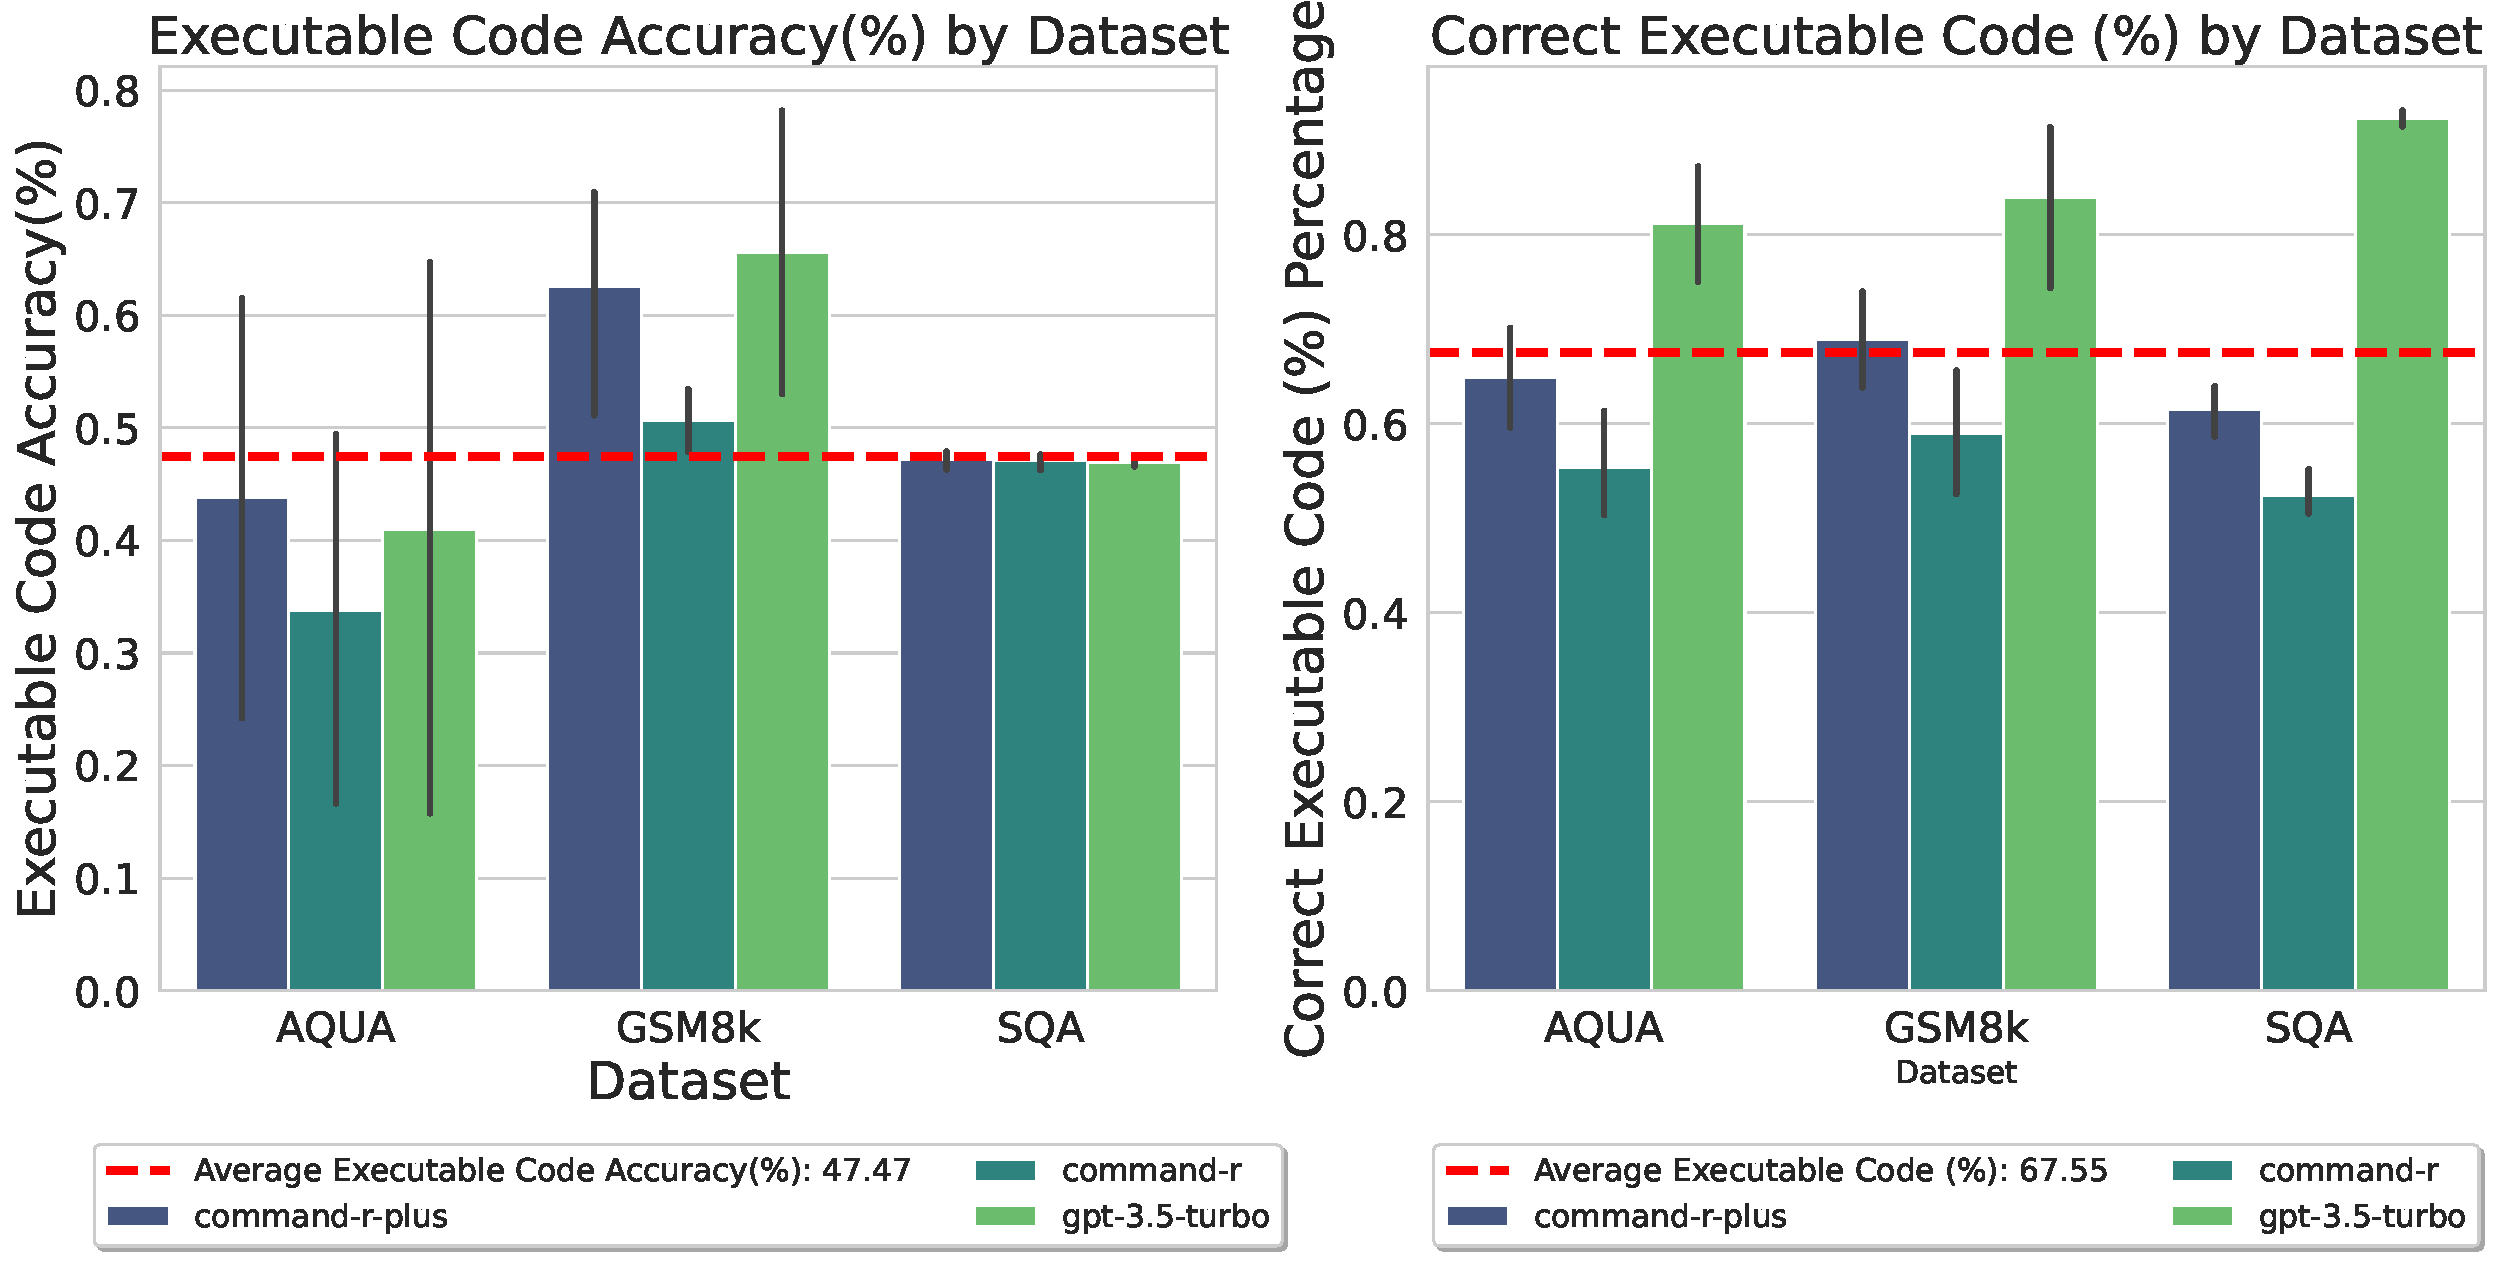
\includegraphics[clip=true,width=\textwidth]{figures/code_exec_by_dataset.pdf}
%         \caption{Code Execution Correctness vs Accuracy}
%     \end{minipage}%
%     \hfill
%     \begin{minipage}[b]{\textwidth}
%         \centering
%         \adjustbox{width=\textwidth,center}{
%         \begin{tabular}{@{}lccc@{}}
%         \toprule
%         \multicolumn{1}{l}{\textbf{Method}} & \multicolumn{1}{l}{GSM8K} & \multicolumn{1}{l}{AQuA} & \multicolumn{1}{l}{StrategyQA} \\ \midrule
%         $\text{CmDR}_\text{\ours}$        & \textbf{52.4} & \textbf{43.7} & \textbf{67.0} \\
%         $\text{CmDR}_\text{plan-only}$    & 24.7          & 35.0          & 65.5          \\
%         $\text{CmDR+}_\text{\ours}$       & 71.4          & \textbf{55.9} & 70.8          \\
%         $\text{CmDR+}_\text{plan-only}$   & 40.7          & 55.1          & \textbf{75.7} \\
%         $\text{GPT-3.5}_\text{\ours}$     & 68.1          & \textbf{55.1} & \textbf{65.5} \\
%         $\text{GPT-3.5}_\text{plan-only}$ & 36.1          & 54.3          & 62.3          \\ \bottomrule
%         \end{tabular}
%         }
%         \caption{The table shows the accuracy of an LLM with {\ours} compared to prompting for a final answer directly after generating (plan-only) a plan $\mathcal{P}$.}
%         \label{tab:plan_only}
%     \end{minipage}
% \end{figure}

\begin{figure}[t!]
    \centering
    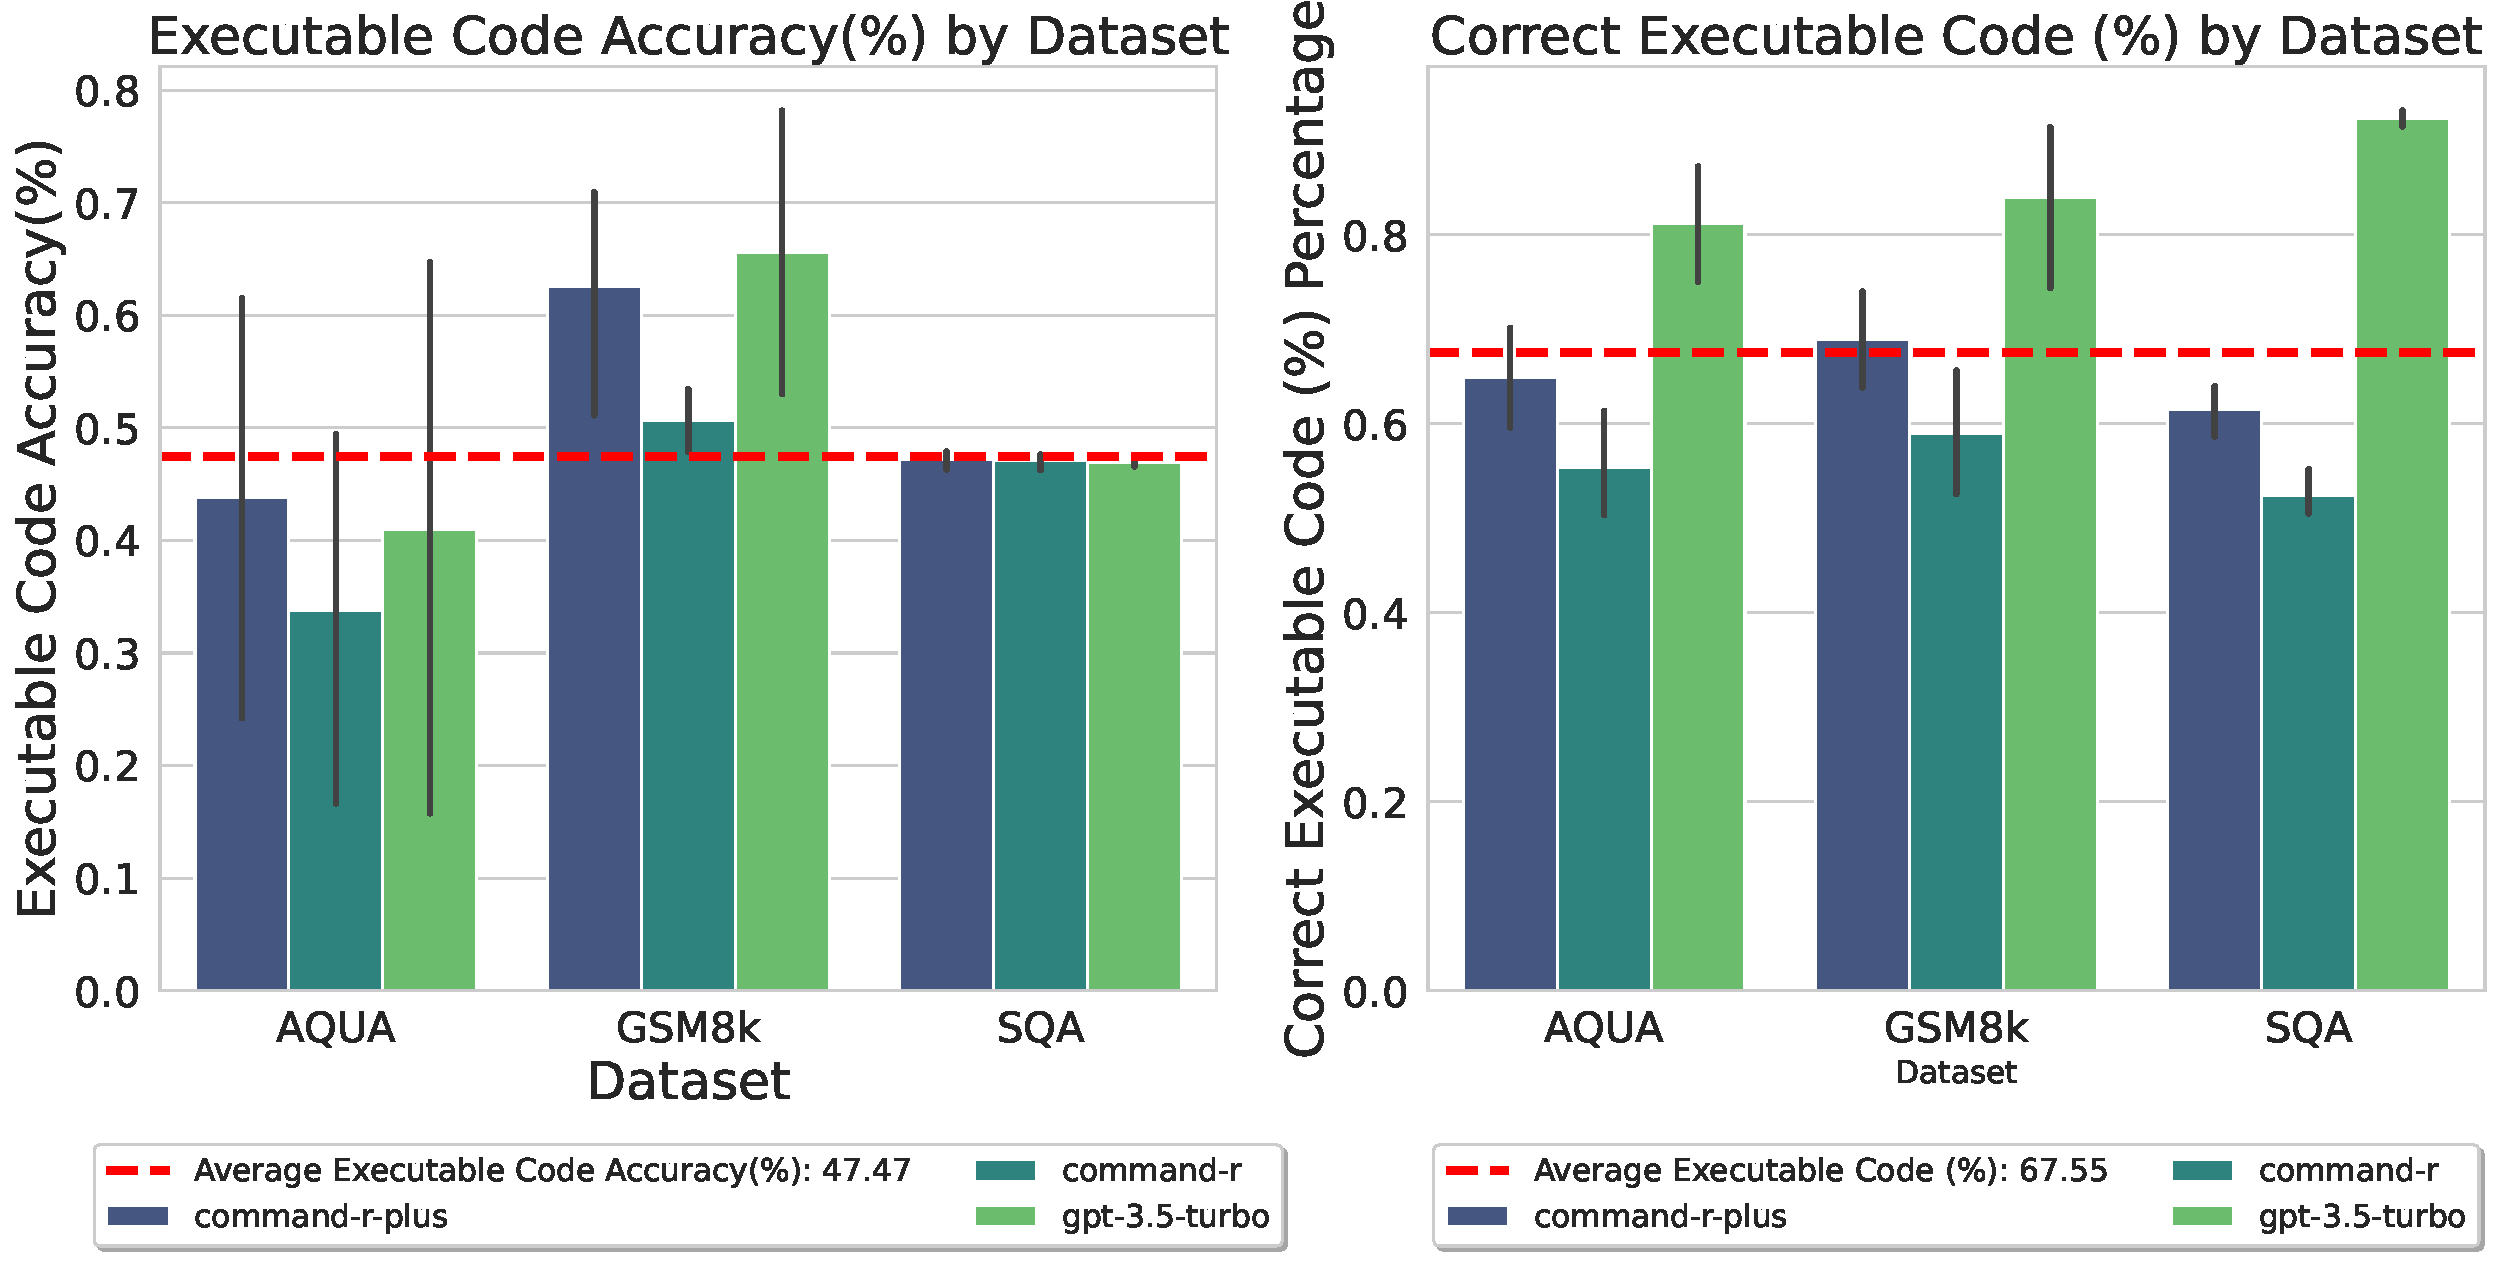
\includegraphics[clip=true,width=\textwidth]{figures/code_exec_by_dataset.pdf}
    \caption{The figure shows the percentage of executable code per model (right) and the accuracy of the executable code when answering the queries (left).}
    \label{fig:code_perc}
\end{figure}

To evaluate {\ours}, we use a set of models of varying sizes on diverse benchmarks, as defined in \cref{sec:ex_setup}. We compare the performance of each model while using {\ours}, CoT and F-CoT prompting. The results for F-CoT and CoT on all the models are computed using the codebase of the original study \citep{DBLP:conf/acl/Xu0P0LH24}.

\paragraph{LLMs for general reasoning} 

Our results, presented in \cref{tab:results_main}, show that using {\ours} allows the LLMs to achieve state-of-the-art results on $7$ out of $9$ datasets, with an average $28\%$ increase over CoT. We can see a clear trend that {\ours} increases the performance compared to CoT and F-CoT for all the models of varying scales. We also see that LLMs that are not explicitly tuned for coding suffer massive degeneracies when using F-CoT. We postulate that they are unable to consistently produce executable programs that satisfy a predefined scheme in F-CoT, thus resulting in an error during execution. This further highlights the value of simulating program execution using an LLM instead of using external solvers.
%
The results show that using {\ours} yields more benefit on datasets that require longer chains of multi-hop and symbolic reasoning, like AQuA and StrategyQA.


\paragraph{LLMs for code generation}

To understand the effect of {\ours} on models tuned for coding, we use GPT3.5 \citep{NEURIPS2020_1457c0d6} as it was the OpenAI suggested succession model for Codex \citep{DBLP:journals/corr/abs-2107-03374} which is used in F-CoT and possesses strong coding capabilities \citep{DBLP:journals/corr/abs-2303-10420}. The results in \cref{tab:results_main} show that using {\ours} is beneficial for models that are tuned for coding and boost the accuracy with a $16\%$ increase over F-CoT and $9\%$ over CoT. The reason is that many natural language queries with non-trivial formalisations are more suited to be tackled with more commonsense soft reasoning than direct code execution. This is evident in \cref{tab:results_main} where {\ours} and CoT are consistently better than F-CoT in StrategyQA, Sports and CLUTRR. 
%
The opposite case of numeric and algorithmic heavy reasoning tasks is also covered by {\ours} as it maintains strong performance similar to F-CoT on MWP problems \cref{tab:results_main}.
%
Consequently, {\ours} allows combining algorithmic formalisation with simulated soft-reasoning, circumventing the pitfalls of using a deterministic external solver while still producing a query formalisation and problem space traversal. 

\subsection{Is simulating search useful?}

To understand if simulating a search over the problem space is useful, we compare the performance of {\ours} where we only generate the \emph{plan} without the subsequent \emph{code} or \emph{search} components. We refer to this framework setup as \emph{plan-only}, which can be seen in \cref{fig:flare} if we were to use only the \emph{plan} for answer generation. We completed this ablation using CmDR, CmDR+, and GPT-3.5, and we used GSM8K, AQuA, and StrategyQA as our baselines. The results in \cref{tab:plan_only} confirm that all of the models suffer massive performance degradation from $61.1 \rightarrow 49.9$ when omitting the \emph{code} and the \emph{search} components of {\ours}. We hypothesise that this is caused by insufficient problem space exploration when using the \emph{plan-only} setting.   
%
Furthermore, we have already seen in \cref{tab:results_main} that in methods, like F-CoT, that do not use simulated problem space exploration for soft-reasoning and only rely on \emph{plan} and \emph{code}, the performance also deteriorates even resulting in a complete breakdown of reasoning over the designated datasets. This can be viewed as a constrained version of {\ours} with \emph{code-only} execution.
%
Consequently, our results show that simulating problem space traversal is highly beneficial as it avoids the pitfalls posed by \emph{plan-only} and \emph{code-only} modes by exploring the problem space more rigorously and soft-reasoning during that traversal instead of using external solvers.

\subsection{Faithful Reasoning Improves Performance}
\begin{table}[t!]
\adjustbox{width=\textwidth}{
\begin{tabular}{@{}lccccc@{}}
\toprule
\textbf{Model} &
  \multicolumn{1}{l}{Avg. Number of Paths} &
  \multicolumn{1}{l}{Avg. \#Hops per path} &
  \multicolumn{1}{l}{Avg. \#Fails per path} &
  \multicolumn{1}{l}{Avg. Total Hops} &
  \multicolumn{1}{l}{Avg. Total Fails} \\ \midrule
\multicolumn{6}{c}{\textbf{Incorrect Answers}}                                                         \\
$\text{Llama-3.1-8B}_\text{\ours}$ & 1.55 & 11.12 & \cellcolor[HTML]{CBCEFB}1.52 & 15.09 & \cellcolor[HTML]{CBCEFB}2.26 \\
$\text{CmDR}_\text{\ours}$             & 1.51 & 6.55  & \cellcolor[HTML]{CBCEFB}0.68 & 10.56 & \cellcolor[HTML]{CBCEFB}1.39 \\
$\text{CmDR+}_\text{\ours}$        & 0.92 & 7.52  & \cellcolor[HTML]{CBCEFB}1.13 & 8.57  & \cellcolor[HTML]{CBCEFB}1.32 \\
GPT-3.5           & 0.68 & 5.22  & \cellcolor[HTML]{CBCEFB}0.71 & 5.32  & \cellcolor[HTML]{CBCEFB}0.74 \\ \midrule
\multicolumn{6}{c}{\textbf{Correct Answers}}                                                           \\ \midrule
$\text{Llama-3.1-8B}_\text{\ours}$ & 1.43 & 9.12  & 0.62                         & 12.36 & 0.96                         \\
$\text{CmDR}_\text{\ours}$             & 1.19 & 7.10  & 0.42                         & 11.29 & 0.66                         \\
$\text{CmDR+}_\text{\ours}$        & 0.97 & 7.19  & 0.42                         & 8.22  & 0.61                         \\
$\text{GPT-3.5}_\text{\ours}$           & 0.82 & 5.65  & 0.26                         & 5.69  & 0.27                         \\ \bottomrule
\end{tabular}
}
\caption{The table depicts the difference in the average explored paths, hops, and fails during the reasoning process, which leads to incorrect or correct answers. The \cellcolor[HTML]{CBCEFB}purple colour illustrates that incorrect reasoning paths have fewer explorations that led to Failed search paths.}
\label{tab:reasoning_stats}
\end{table}

As described in \cref{sec:method}, using {\ours} allows us to measure the faithfulness of the LLM reasoning process by comparing the simulated problem space traversals ${\Phi}^\prime_\text{\emph{gen}}$ with actual traces ${\Phi}^\prime$ produced from a symbolic Prolog solver. To do this, we initially compute the percentage of syntactically correct executable code each LLM produces. We can see from the right part of \cref{fig:code_perc} that all of the models are capable of producing correct executable Prolog code in $67\%$ of cases on average and $\geq 50\%$ of cases at the very least. This shows that the simulated searches ${\Phi}^\prime_\text{\emph{gen}}$ can be considered a representative sample that will be further used to accurately measure the faithfulness of the simulated search w.r.t. the generated code. After measuring the reasoning faithfulness for each model, we want to understand what impact it has on the performance of the LLM. In \cref{fig:faith_vs_acc}, we segment the models w.r.t. their ROUGE-Lsum scores. The results show that model performance is strongly positively correlated with reasoning faithfulness. 
%
However, we also observe in the left part of \cref{fig:code_perc} that executing semantically precise code results in an accurate answer only in $47\%$ of cases on average. Indeed, having a simulated search trace with a ROUGE-Lsum faithfulness score of $1$, would be equivalent to simply executing the program as proposed in F-CoT. Yet we have priorly shown that F-CoT struggles with reasoning tasks that are hard to formalise and require multi-hop commonsense and soft reasoning.
%
These two discoveries show that optimal LLM reasoning, conditioned on a search in the problem space, should be increasingly faithful toward the facts, relations and the search strategy defined within the code while simultaneously maintaining the capability for soft-reasoning along more abstractly defined concepts. Our results show that {\ours} allows LLMs to maintain a similar reasoning capacity.

\subsection{What is important during the search?}
% Please add the following required packages to your document preamble:
% \usepackage{booktabs}
\begin{table}[t!]
\adjustbox{width=\textwidth}{
\begin{tabular}{@{}lccc@{}}
\toprule
\textbf{Model} & \multicolumn{1}{r}{Unique Explorations (\%) in Search} & \multicolumn{1}{l}{Relation overlap (\%)} & \multicolumn{1}{r}{Unused Code relations (\%)} \\ \midrule
\multicolumn{4}{c}{\textbf{Correct Answers}}   \\ \midrule
$\text{Llama-3.1-8B}_\text{\ours}$   & 74.14   & 43.65  & 5.73  \\
$\text{CmDR}_\text{\ours}$               & 59.06   & 35.96  & 4.02  \\
$\text{CmDR+}_\text{\ours}$              & 64.30   & 34.47  & 4.54  \\
$\text{GPT-3.5}_\text{\ours}$             & 64.46   & 37.55  & 1.90  \\ \midrule
\multicolumn{4}{c}{\textbf{Incorrect Answers}} \\ \midrule
$\text{Llama-3.1-8B}_\text{\ours}$   & 54.69   & 35.04  & 9.28  \\
$\text{CmDR}_\text{\ours}$               & 54.50   & 32.76  & 6.23  \\
$\text{CmDR+}_\text{\ours}$              & 44.12   & 24.98  & 8.22  \\
$\text{GPT-3.5}_\text{\ours}$             & 36.02   & 24.44  & 6.94  \\ \bottomrule
\end{tabular}
}
\caption{The table shows how the percentage of unique emergent inferences in search, overlapping relations between code and search, and unused relations in code impact answer correctness.}
\label{tab:reasoning_stats_deep}
\end{table}

We expand the analysis of the simulated search traces to detect the reasons which can lead to optimal reasoning within an LLM. For this purpose, we calculate several statistics, like the average number of explored paths, average and total hops and failures per path, for each model during the simulated traversal. The failure in a path is an invalidation of a solution for a sub-goal explored during the search, which is used for backtracking, as explained in \cref{sec:method}. Calculating these statistics is simple as the \emph{search} component of {\ours}, seen in \cref{fig:flare}, is a structured simulation of a Prolog trace, where each line contains a hop of reasoning inference.
%
We split these statistics for the reasoning paths that lead to correct or incorrect outcomes. Our results in \cref{tab:reasoning_stats} show that LLM performance and reasoning optimally are not directly connected to the amount of explored paths or multi-hop inferences per path. We also see that traces that lead to incorrect answers have a higher number of failures per path and in total. We explain this phenomenon with the hypothesis that LLMs with traces that were optimal for reasoning and led to correct answers could skip exploring degenerate solutions due to strong commonsense reasoning capabilities.
%
Further analyses focus on identifying inconsistencies and failure modes (\cref{subsec:reasoning_inc}). By comparing relations in code with those in search traces, we measure emergent hallucinations and unused relations, highlighting areas of sub-optimal reasoning. Additionally, we assess the uniqueness of emergent facts per inference hop, which indicates the extent of problem-space exploration (\cref{tab:reasoning_stats_deep}).
%
The results in \cref{tab:reasoning_stats_deep} show consistently over each model that, on average, traces that lead to correct answers had a higher percentage of unique emergent facts and overlap in the relations used between the code and search, while the portion of underutilized relations was lower. This means that optimal reasoning with an LLM requires a great degree of problem-space exploration with fewer relation hallucinations during the search and more relation utilization from the defined code. This aligns with our prior discoveries, which show a strong correlation between simulated search faithfulness towards the formalised code and model performance. Our framework {\ours} has these reasoning patterns ingrained within its inference pipeline. 

\begin{figure}[t!]
    \centering
    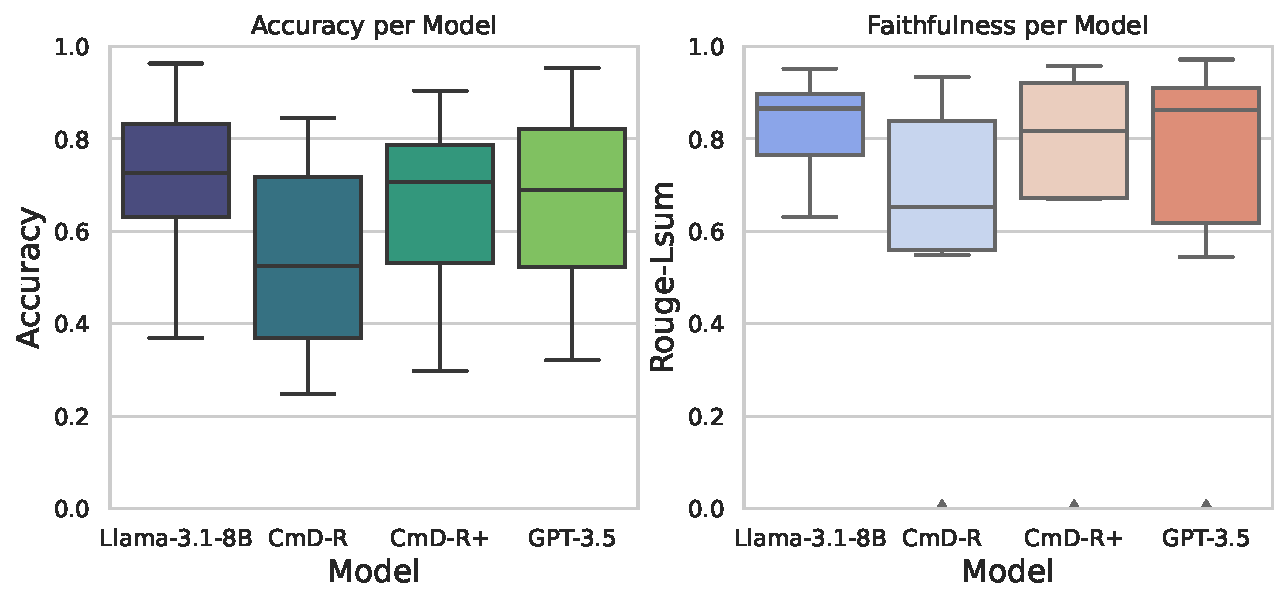
\includegraphics[clip=true,width=0.935\textwidth]{figures/effect_of_scale.pdf}
    \caption{The effect of the model parameter scale from 8B to 100B+ on model accuracy (left) and faithfulness (right).}
    \label{fig:effect_of_scale}
\end{figure}

\subsection{The effect of scale}
% Please add the following required packages to your document preamble:
% \usepackage{booktabs}
\begin{table}[t!]
\adjustbox{width=\textwidth}{
\begin{tabular}{@{}lcccc@{}}
\toprule
\textbf{Model} &
  \multicolumn{1}{l}{Avg. hops per Paths} &
  \multicolumn{1}{r}{Hallucination (\%)} &
  \multicolumn{1}{r}{Unutilised knowledge (\%)} \\ \midrule
Llama-3.1-8B   & 9.4 & 63.3 & 62.9  \\
CmDR           & 6.7 & 54.7 & 56.9 \\
CmDR+         & 7.2 & 54.3 & 56.3 \\
GPT-3.5       & 5.5 & 49.3 & 52.1 \\ \bottomrule
\end{tabular}
}
\caption{The table shows the changes in simulated search statistics when using {\ours} w.r.t model scale from 8B to 100B+. Hallucinations refer to facts and predicates only used in trace, while unutilised knowledge relates to the facts and relations only seen in the code. }
\label{tab:scale_effect}
\end{table}

We want to assess the impact of the number of parameters in the model on the overall performance and faithfulness. The results in \cref{fig:effect_of_scale} show no precise relation between model scale, performance and faithfulness. However, scaled models from the same family, i.e. CmDR (30B) and CmDR+ (100B), show improvements in reasoning faithfulness and model performance. We can also see in  \cref{tab:scale_effect} that as the model size increases, the average number of hops and the portion of hallucinations and unutilised knowledge decreases. This further confirms our prior assumptions that models with strong commonsense soft-reasoning capabilities can skip steps during the search while maintaining the knowledge and structure of the traversal strategy outlined in the code. 

\section{Related Work}
\label{sec:related}

\paragraph{Reasoning in Natural Language}
Few-shot prompting \citep{DBLP:conf/nips/BrownMRSKDNSSAA20} has been shown to be an effective approach for increasing the reasoning capabilities of LLMs in natural language generation \citep{DBLP:journals/corr/abs-2102-01672, DBLP:conf/acl/ReifIYCCW22,DBLP:conf/iclr/SanhWRBSACSRDBX22}. LLM reasoning can be further enhanced with prompting techniques such as CoT \citep{wei2022chain}, which attempts to segment reasoning into explicitly written intermediate steps. Concurrent work has also proposed that models \emph{``think step by step''} \citep{DBLP:conf/nips/KojimaGRMI22}, or divide the problem into subtasks before the solution \citep[Least-to-Most]{DBLP:conf/iclr/ZhouSHWS0SCBLC23}. These approaches have been shown to suffer from arithmetic inaccuracies \citep{DBLP:conf/nips/LewkowyczADDMRS22, DBLP:conf/nips/HendrycksBKABTS21} and reasoning inconsistencies \citep{DBLP:journals/corr/abs-2209-07686}. Further attempts have been made to add a planning stage before reasoning by dividing the process into recursive plan formulation and execution steps \citep{DBLP:conf/iclr/YaoZYDSN023,DBLP:conf/acl/WangXLHLLL23}. The \emph{plan} generation step in {\ours} is a hybrid technique inspired by these methods but focused on generating a natural language strategy for formalising the query into code. 
%
\paragraph{Reasoning with Search}

Several lines of work propose using techniques to expand the reasoning paths over the problem space. Self-consistency decoding \citep{DBLP:conf/iclr/0002WSLCNCZ23} is an approach used to sample many natural language reasoning paths and take a majority vote for an answer. Another popular approach is Tree-of-Thoughts (ToT, \citet{DBLP:conf/nips/YaoYZS00N23}), which proposes to explore the problem space with reasoning similar to a tree traversal, where each state is created and evaluated using an LLM. Similar techniques try to adapt symbolic search approaches akin to DFS, BFS \citep{DBLP:conf/aaai/BestaBKGPGGLNNH24}, A$^*$ \citep{DBLP:journals/corr/abs-2402-14083} or other combinations \citep{DBLP:journals/corr/abs-2404-03683} with direct tuning \citep{DBLP:journals/corr/abs-2402-14083}, imitation training \citep{DBLP:conf/nips/YangSAN22} or few-shot prompting \citep{DBLP:journals/corr/abs-2404-01230}. It must be noted that all of these techniques have only been tested in constrained mathematical puzzle-solving and algorithmic domains like the 24 Game \citep{DBLP:conf/nips/YangSAN22}, Countdown \citep{wiki:Countdown}, Sorting \citep{DBLP:conf/aaai/BestaBKGPGGLNNH24}, maze solving \citep{DBLP:conf/nips/YangSAN22}, Sokoban \citep{DBLP:journals/corr/abs-2402-14083} and others.
%
Although the \emph{search} component of {\ours} has some similarities to these techniques, we argue that our method allows for generalistic reasoning with interpretable multi-hop search through iterative logic-based problem space exploration.

\paragraph{Reasoning with Formalisation}

Another line of research has tried formalising natural language queries into code \citep{DBLP:conf/icml/GaoMZ00YCN23,DBLP:conf/icml/0002LZCHSL0XI24} or pseudo-code \citep{DBLP:journals/corr/abs-2404-02575,DBLP:journals/corr/abs-2404-03683}. This allows the translation of the query into a strict structure and offloads the reasoning and search components to deterministic solvers like Python \cite{DBLP:journals/tmlr/ChenM0C23}, PDDL \cite{DBLP:conf/acl/Xu0P0LH24, DBLP:journals/corr/abs-2304-11477}, DataLog \cite{DBLP:conf/acl/Xu0P0LH24} and others. While models are reasonably capable of synthesising programs \citep{DBLP:journals/corr/abs-2108-07732, DBLP:conf/iclr/NijkampPHTWZSX23} and benefit from the use of code in numerical and algorithmic reasoning settings \citep{DBLP:journals/tmlr/ChenM0C23,DBLP:conf/icml/GaoMZ00YCN23}, the usage of code for general QA has not been rigorously explored. The reasons are that formalisation from natural language into a strict and executable code is challenging \citep{DBLP:conf/nips/WuJLRSJS22}, following the exact syntactic constraints of the programming language not abundantly used during pre-training is onerous \citep{DBLP:journals/corr/abs-2404-00971} and can require models explicitly tuned for coding \citep{DBLP:journals/corr/abs-2107-03374}. Using an external solver for reasoning also limits the capability for soft reasoning in commonsense knowledge and implications. Although we formalise the natural language query into a logic programming Prolog program during the \emph{code} generation part of {\ours}, we do not explicitly require the code to be executable and do not use external solvers during inference. This allows for the further use of the LLM for soft-reasoning to simulate code execution in a logic-based problem space traversal similar to Prolog while circumventing the need for code tuning a generalist model.
%

\paragraph{Reasoning Faithfulness}

An explanation is considered \emph{faithful} if it explicitly and accurately describes the reasoning process of the model during inference \citep{DBLP:conf/dsaa/GilpinBYBSK18, DBLP:conf/acl/JacoviG20}. In the context of prompting techniques such as CoT, we are interested in the faithfulness of the intermediate reasoning chains towards the final output. Faithful intermediate reasoning chains should not just look \emph{plausible} \citep{herman2017promise} but have exact reflections of the problem exploration and reasoning used to arrive at the final answer. Natural language reasoning chains prevalent in CoT and similar methods are shown to be unfaithful, either masking the reasoning biases \citep{DBLP:conf/nips/TurpinMPB23} of the model or outright ignoring the intermediate reasoning \citep{DBLP:journals/corr/abs-2307-13702}. In {\ours}, we introduce a method to seamlessly measure the faithfulness of the final outcome w.r.t. completed search.

\section{Conclusion}

This work introduces {\ours}, a novel approach for logic-aided interpretable formalisation and reasoning with simulated search over the problem space. We show that models of varying scales obtain state-of-the-art results compared to prompting paradigms like CoT and F-CoT. We further pinpoint that using {\ours} allows us to perform soft-reasoning with simulated search, making it flexible for diverse reasoning benchmarks. We introduce a method to measure model reasoning faithfulness w.r.t. the problem formalization ingrained within {\ours}. Our results show that model performance is positively correlated with the faithfulness of the reasoning process. The systematic studies of the method show the benefits of using simulated search compared to natural language reasoning and external symbolic solvers. We further show that using {\ours} allows us to interpretably and rigorously detect hallucinations and sub-optimal and inconsistent reasoning patterns.

\section*{Reproducibility Report}

To reproduce the results of our study, we provide the complete codebase, processing pipelines and prompts for each dataset. The only model hyper-parameter we explicitly fix is the temperature for greedy decoding. We also make the inference of all of the models using {\ours}, F-CoT and CoT across all of the datasets publicly available for further experimentation and exploration.

\section*{Acknowledgments}
$\begin{array}{l}
\includegraphics[width=1cm]{figures/LOGO_ERC-FLAG_EU.jpg} \end{array}$ 
%
Erik is partially funded by a DFF Sapere Aude research leader grant under grant agreement No 0171-00034B, as well as by a NEC PhD fellowship.
%
Pasquale was partially funded by ELIAI (The Edinburgh Laboratory for Integrated Artificial Intelligence), EPSRC (grant no.\ EP/W002876/1), an industry grant from Cisco, and a donation from Accenture LLP.
%
Isabelle's research is partially funded by the European Union (ERC, ExplainYourself, 101077481).
%
This work was further supported by by the Pioneer Centre for AI, DNRF grant number P1, the Edinburgh International Data Facility (EIDF) and the Data-Driven Innovation Programme at the University of Edinburgh.
%

\bibliography{references}
\bibliographystyle{iclr2025_conference}
\newpage{}
\appendix
\section{Appendix}
\label{append:prompts}

\subsection{LLM Prompts}
We define straight-forward prompts for generating \emph{plan}, \emph{code} and \emph{search} simulation in {\ours}, which can be observed in \cref{tab:prompts}. 

\subsection{Dataset Statistics}

The datasets used in this study encompass a variety of domains, specifically targeting the performance of the models in interpreting Math Word Problems, multi-hop question answering, and relational inference. Table \ref{tab:data_stat} provides a detailed breakdown of each dataset, including the number of few-shot in-context samples (shots), the number of test samples, and representative examples from each dataset. The datasets provide a comprehensive basis for evaluating the models' abilities to handle complex tasks across different domains, facilitating an in-depth analysis of model performance under few-shot conditions.


\clearpage
\onecolumn  % Switch to one column before strip environment
\section{Prompts}
\label{appendix_sec:agent_prompts}

\subsection{Offline Prompts}
\label{sec:offline_prompts}
\begin{prompt}[title={Reader}]
 \textbf{\# Instruction} \\
\\
Your task is to construct an RDF (Resource Description Framework) graph from the given passages and named entity lists. \\
Respond with a JSON list of triples, with each triple representing a relationship in the RDF graph. \\
Pay attention to the following requirements: \\
- Each triple should contain at least one, but preferably two, of the named entities in the list for each passage. \\
- Clearly resolve pronouns to their specific names to maintain clarity. \\
\\
Convert the paragraph into a JSON dict containing a named entity list and a triple list. \\
\\
\ \textbf{\# Demonstration \#1} \\
\\
Paragraph: \\
``` \\
Magic Johnson \\
\\
After winning a national championship with Michigan State in 1979, Johnson was selected first overall in the 1979 NBA draft by the Lakers, leading the team to five NBA championships during their "Showtime" era. \\
``` \\
\{\{"named\_entities": ["Michigan State", "national championship", "1979", "Magic Johnson", \\ "National Basketball Association", "Los Angeles Lakers", "NBA Championship"]\}\} \\
\{\{ \\
    "triples": [ \\
        ("Magic Johnson", "member of sports team", "Michigan State"), \\
        ("Michigan State", "award", "national championship"), \\
        ("Michigan State", "award date", "1979"), \\
        ("Magic Johnson", "draft pick number", "1"), \\
        ("Magic Johnson", "drafted in", "1979"), \\
        ("Magic Johnson", "drafted by", "Los Angeles Lakers"), \\
        ("Magic Johnson", "member of sports team", "Los Angeles Lakers"), \\
        ("Magic Johnson", "league", "National Basketball Association"), \\
        ("Los Angeles Lakers", "league", "National Basketball Association"), \\
        ("Los Angeles Lakers", "award received", "NBA Championship"), \\
    ] \\
\}\} \\
``` \\
\\
\ \textbf{\# Demonstration \#2} \\
\\
Paragraph: \\
``` \\
Elden Ring \\
\\
Elden Ring is a 2022 action role-playing game developed by FromSoftware. It was directed by Hidetaka Miyazaki with worldbuilding provided by American fantasy writer George R. R. Martin. \\
``` \\
\{\{"named\_entities": ["Elden Ring", "2022", "Role-playing video game", "FromSoftware", "Hidetaka Miyazaki", "United States of America", "fantasy", "George R. R. Martin"]\}\} \\
\{\{ \\
    "triples": [ \\
        ("Elden Ring", "publication", "2022"), \\
        ("Elden Ring", "genre", "action role-playing game"), \\
        ("Elden Ring", "publisher", "FromSoftware"), \\
        ("Elden Ring", "director", "Hidetaka Miyazaki"), \\
        ("Elden Ring", "screenwriter", "George R. R. Martin"), \\
        ("George R. R. Martin", "country of citizenship", "United States of America"), \\
        ("George R. R. Martin", "genre", "fantasy"), \\
    ] \\
\}\} \\
\\
\\
\ \textbf{\# Input} \\
\\
Convert the paragraph into a JSON dict, it has a named entity list and a triple list. \\
\\
Paragraph: \\
``` \\
\textbf{$\{$wiki\_title$\}$} \\
\\
\textbf{$\{$passage$\}$}\\
\end{prompt}

\subsection{Online Retrieval Prompts}
\label{subsec:online_retrieval_prompts}

The \textcolor{blue}{blue}-highlighted portions of the Reader prompt below indicate additional text that is only required when the Gist Memory $\mathcal{G}^{(n)}$ is active. When Gist Memory is inactive, these blue sections should be omitted, and the $\{$triples$\}$ parameter should be left empty.

\begin{prompt}[title={Reader with and without Gist Memory }]
Your task is to find facts that help answer an input question. \\
\\
You should present these facts as knowlege triples, which are structured as ("subject", "predicate", "object"). \\
Example: \\
Question: When was Neville A. Stanton's employer founded? \\
Facts: ("Neville A. Stanton", "employer", "University of Southampton"), ("University of Southampton", "founded in", "1862") \\
\\
\\
Now you are given some documents:\\
\textbf{$\{$docs$\}$} \\
\\
\\
Based on these documents \textcolor{blue}{and some preliminary facts provided below}, \\ find additional supporting fact(s) that may help answer the following question. \\
 \\
Note: if the information you are given is insufficient, output only the relevant facts you can find.\\
\\
Question: \textbf{$\{$query$\}$} \\
Facts: \textcolor{blue}{\textbf{$\{$triples$\}$}} \\
\end{prompt}

\begin{prompt}[title={Reasoning for Termination}]
\ \textbf{\# Task Description:} \\
You are given an input question and a set of known facts:\\
Question: \textbf{$\{$query$\}$} \\
Facts: \textbf{$\{$triples$\}$} \\
\\
Your reply must follow the required format:\\
1. If the provided facts contain the answer to the question, your should reply as follows:\\
Answerable: Yes\\
Answer: ...\\
\\
2. If not, you should explain why and reply as follows:\\
Answerable: No\\
Why: ...\\
\\
\ \textbf{\# Your reply:} \\
\end{prompt}


\begin{prompt}[title={Query Re-writing}]
\ \textbf{\# Task Description:} \\
You will be presented with an input question and a set of known facts. \\
These facts might be insufficient for answering the question for some reason. \\
Your task is to analyze the question given the provided facts and 
determine what else information is needed for the next step. \\
\\
\ \textbf{\# Example:} \\
Question: What region of the state where Guy Shepherdson was born, contains SMA Negeri 68?\\
Facts: ("Guy Shepherdson", "born in", "Jakarta")\\
Reason: The provided facts only indicate that Guy Shepherdson was born in Jakarta, but they do not provide any information about the region of the state that contains SMA Negeri 68. \\
Next Question: What region of Jakarta contains SMA Negeri 68? \\
\\
\ \textbf{\# Your Task:} \\
Question: \textbf{$\{$query$\}$} \\
Facts: \textbf{$\{$triples$\}$} \\
Reason: \textbf{$\{$reason$\}$} \\
\\
Next Question:
\end{prompt}

\subsection{Online Question Answering Prompts}

The following prompt with retrieved passages combines the QA generation prompts from \citeauthor{Gutierrez2024} and \citeauthor{Wang2024}. For the variation without retrieved passages, we omit the preamble and only include the instruction, highlighted in \textcolor{purple}{purple} .

\begin{prompt}[title={Retrieved Passages with In-context Example}]
As an advanced reading comprehension assistant, your task is to analyze text passages and corresponding questions meticulously, with the aim of providing the correct answer. \\
==================\\
For example:\\
==================\\
Wikipedia Title: Edward L. Cahn \\
Edward L. Cahn (February 12, 1899 – August 25, 1963) was an American film director.\\
\\
Wikipedia Title: Laughter in Hell \\
Laughter in Hell is a 1933 American Pre-Code drama film directed by Edward L. Cahn and starring Pat O'Brien. The film's title was typical of the sensationalistic titles of many Pre-Code films. Adapted from the 1932 novel of the same name buy Jim Tully, the film was inspired in part by "I Am a Fugitive from a Chain Gang" and was part of a series of films depicting men in chain gangs following the success of that film. O'Brien plays a railroad engineer who kills his wife and her lover in a jealous rage and is sent to prison. The movie received a mixed review in "The New York Times" upon its release. Although long considered lost, the film was recently preserved and was screened at the American Cinematheque in Hollywood, CA in October 2012. The dead man's brother ends up being the warden of the prison and subjects O'Brien's character to significant abuse. O'Brien and several other characters revolt, killing the warden and escaping from the prison. The film drew controversy for its lynching scene where several black men were hanged. Contrary to reports, only blacks were hung in this scene, though the actual executions occurred off-camera (we see instead reaction shots of the guards and other prisoners). The "New Age" (an African American weekly newspaper) film critic praised the scene for being courageous enough to depict the atrocities that were occurring in some southern states. \\
\\
Wikipedia Title: Theodred II (Bishop of Elmham) \\
Theodred II was a medieval Bishop of Elmham. The date of Theodred's consecration unknown, but the date of his death was sometime between 995 and 997. \\
\\
Wikipedia Title: Etan Boritzer \\
Etan Boritzer( born 1950) is an American writer of children 's literature who is best known for his book" What is God?" first published in 1989. His best selling" What is?" illustrated children's book series on character education and difficult subjects for children is a popular teaching guide for parents, teachers and child- life professionals. Boritzer gained national critical acclaim after" What is God?" was published in 1989 although the book has caused controversy from religious fundamentalists for its universalist views. The other current books in the" What is?" series include What is Love?, What is Death?, What is Beautiful?, What is Funny?, What is Right?, What is Peace?, What is Money?, What is Dreaming?, What is a Friend?, What is True?, What is a Family?, What is a Feeling?" The series is now also translated into 15 languages. Boritzer was first published in 1963 at the age of 13 when he wrote an essay in his English class at Wade Junior High School in the Bronx, New York on the assassination of John F. Kennedy. His essay was included in a special anthology by New York City public school children compiled and published by the New York City Department of Education. \\
\\
Wikipedia Title: Peter Levin \\
Peter Levin is an American director of film, television and theatre. \\
\\
Question: When did the director of film Laughter In Hell die? \\
Answer: August 25, 1963. \\
================== \\
\textcolor{purple}{Given the following text passages and questions, please present a concise, definitive answer, devoid of additional elaborations, and of maximum length of 6 words.} \\
================== \\
\\
Wikipedia Title : \textbf{$\{$title$\}$}
\textbf{$\{$text$\}$} \texttt{for each retrieved passage} ...  \\
Question: \textbf{$\{$question$\}$} \\
\\
Answer:
\end{prompt}

\label{subsec:online_qa_prompts}
\begin{prompt}[title={No Retrieved Passages}]
\textcolor{purple}{Given the following question, please present a concise, definitive answer, devoid of additional elaborations, and of maximum length of 6 words.} \\
\\
Question: \textbf{$\{$question$\}$} \\
\\
Answer:
\end{prompt}

% Please add the following required packages to your document preamble:
% \usepackage{booktabs}
% \usepackage{multirow}
\begin{table}[t!]
\adjustbox{width=\textwidth}{
\begin{tabular}{@{}ccccc@{}}
\toprule
Domain &
  Dataset &
  Shots &
  Test Samples &
  Example \\ \midrule
\multirow{4}{*}{\begin{tabular}[c]{@{}c@{}}Math \\ Word \\ Problems\end{tabular}} &
  GSM8K &
  8 &
  1,319 &
  \begin{tabular}[c]{@{}c@{}}Q: A robe takes 2 bolts of blue fiber and half that much white fiber.  \\ How many bolts in total does it take?\\ A: 3\end{tabular} \\
 &
  SVAMP &
  8 &
  1,000 &
  Q: Dan had \$3 left with him after he bought a candy bar. If he had \$4 at the start, how much did the candy bar cost?A: 1 \\
 &
  MultiArith &
  8 &
  600 &
  \begin{tabular}[c]{@{}c@{}}Q: A pet store had 13 siamese cats and 5 house cats. During a sale they sold 10 cats. \\ How many cats do they have left? \\ A: 8\end{tabular} \\
 &
  ASDiv &
  8 &
  2,096 &
  \begin{tabular}[c]{@{}c@{}}Q: Adam has five more apples than Jackie. Jackie has nine apples. How many apples does Adam have?\\ \\ A: 14\end{tabular} \\
\multicolumn{1}{l}{} &
  AQuA &
  8 &
  254 &
  \begin{tabular}[c]{@{}c@{}}Q: A man walks at 5 kmph for 6 hrs and at 4 kmph for 12 hrs. His average speed is\\ Answer option: A)4 1/3 km/h, B)7 2/3 km/h, C)9 ½ km/h, D)8 km/h, E)81 km/h\\ A: A\end{tabular} \\ \midrule
\begin{tabular}[c]{@{}c@{}}Multi- \\ hop \\ QA\end{tabular} &
  StrategyQA &
  6 &
  2,290 &
  \begin{tabular}[c]{@{}c@{}}Q: Did Aristotle use a laptop? \\ A: False\end{tabular} \\
 &
  \begin{tabular}[c]{@{}c@{}}Date \\ Understanding\end{tabular} &
  10 &
  359 &
  \begin{tabular}[c]{@{}c@{}}Q: Yesterday was April 30, 2021. What is the date tomorrow in MM/DD/YYYY? \\ A: "05/02/2021"\end{tabular} \\
 &
  \begin{tabular}[c]{@{}c@{}}Sports \\ Understanding\end{tabular} &
  10 &
  977 &
  \begin{tabular}[c]{@{}c@{}}Q: Is the following sentence plausible? Lionel Messi was called for icing? \\ A: False\end{tabular} \\ \midrule
\begin{tabular}[c]{@{}c@{}}Relational \\ Inference\end{tabular} &
  CLUTRR &
  8 &
  1,042 &
  \begin{tabular}[c]{@{}c@{}}Q: [Carlos] is [Clarence]'s brother. [Carlos] and his sister, [Annie], went shopping. \\ asked her mom [Valerie] if she wanted anything, but [Valerie] said no. \\ How is [Valerie] related to [Clarence]? \\ A: "mother"\end{tabular} \\ \bottomrule
\end{tabular}
}
\caption{The statistics and examples of the datasets used in benchmarking. Shots refers to the number of few-shot in-context samples used during benchmarking.}
\label{tab:data_stat}
\end{table}





\end{document}
